%% BATON manuscript — Elsevier elsarticle, prepared for Omega
%% Build: pdflatex main && bibtex main && pdflatex main && pdflatex main
%%
%% Double-blind toggle: \anontrue for an anonymised copy,
%% \anonfalse for the submission copy with author identity.

%% Submission copy is anonymised: author identity lives in the cover
%% letter (cover_letter.tex). Flip to \anonfalse for a named copy.
\newif\ifanon
\anontrue

\documentclass[preprint,12pt]{elsarticle}

\usepackage{amsmath,amssymb,amsthm}
\usepackage{booktabs}
\usepackage{graphicx}
\usepackage{algorithm}
\usepackage{algpseudocode}
\usepackage{tikz}
\usetikzlibrary{shapes.geometric,arrows.meta,positioning}
\usepackage[colorlinks=true,allcolors=blue!50!black]{hyperref}

\newtheorem{theorem}{Theorem}
\newtheorem{proposition}[theorem]{Proposition}
\newtheorem{corollary}[theorem]{Corollary}
\newtheorem{lemma}[theorem]{Lemma}
\theoremstyle{definition}
\newtheorem{assumption}{Assumption}
\theoremstyle{remark}
\newtheorem{remark}{Remark}

% float placement: several figures are near-full-page, so relax the
% defaults or they queue behind one another and dump after the references
\renewcommand{\topfraction}{0.9}
\renewcommand{\textfraction}{0.07}
\renewcommand{\floatpagefraction}{0.66}

% elsarticle's pprintTitle footer wraps an \hbox to \textwidth followed by a
% stray end-of-line space, overfull by one \footnotesize space — rebuild the
% footer without the inner box
\makeatletter
\def\ps@pprintTitle{%
  \let\@oddhead\@empty
  \let\@evenhead\@empty
  \def\@oddfoot{\footnotesize\itshape
    Preprint submitted to \ifx\@journal\@empty Elsevier\else\@journal\fi
    \hfill\@date}%
  \let\@evenfoot\@oddfoot}
\makeatother

% numbers regenerated from result files by make_tables.py — do not hand-edit
% generated by make_tables.py — do not hand-edit
\newcommand{\batonGrandBest}{53.4\%}
\newcommand{\batonWDpxlN}{235/240}
\newcommand{\batonWDpxlP}{$p \le 10^{-39}$}
\newcommand{\batonWHoN}{239/240}
\newcommand{\batonWHoP}{$p \le 10^{-40}$}
\newcommand{\batonWPiThreeN}{240/240}
\newcommand{\batonWPiThreeP}{$p \le 10^{-40}$}
\newcommand{\batonWRestockN}{221/240}
\newcommand{\batonWRestockP}{$p \le 10^{-38}$}
\newcommand{\batonWRolloutN}{240/240}
\newcommand{\batonWRolloutP}{$p \le 10^{-40}$}
\newcommand{\batonWThreshN}{240/240}
\newcommand{\batonWThreshP}{$p \le 10^{-40}$}
\newcommand{\certBeatN}{17/40}
\newcommand{\certGap}{9.34\%}
\newcommand{\certGapHighs}{11.03\%}
\newcommand{\certGapMax}{12.55\%}
\newcommand{\ctdBaton}{51.9\%}
\newcommand{\ctdVOne}{0.0\%}
\newcommand{\dearSbBaton}{41.9\%}
\newcommand{\dearSbOrc}{24.8\%}
\newcommand{\dearSbThresh}{7.3\%}
\newcommand{\nCity}{19}
\newcommand{\rlBatonHo}{33.9\%}
\newcommand{\rlBest}{28.7\%}
\newcommand{\rlWinN}{40/50}
\newcommand{\rlWinP}{$p \le 10^{-8}$}
\newcommand{\shopTravelSaving}{25.9\%}
\newcommand{\svCityBaton}{10.8\%}
\newcommand{\svCuiBaton}{51.6\%}
\newcommand{\svCuiHo}{20.7\%}
\newcommand{\svCuiOrc}{43.2\%}
\newcommand{\svCuiThresh}{16.6\%}
\newcommand{\svDetBaton}{27.8\%}
\newcommand{\svDetHo}{26.1\%}
\newcommand{\svDetOrc}{40.7\%}
\newcommand{\svDetThresh}{24.8\%}
\newcommand{\svGounarisBaton}{52.8\%}
\newcommand{\svGounarisHo}{21.2\%}
\newcommand{\svGounarisOrc}{43.5\%}
\newcommand{\svGounarisThresh}{17.0\%}
\newcommand{\svMDROBaton}{44.3\%}
\newcommand{\svMDROHo}{11.9\%}
\newcommand{\svMDROOrc}{42.2\%}
\newcommand{\svMDROThresh}{-1.8\%}
\newcommand{\svSAABaton}{53.4\%}
\newcommand{\svSAAHo}{20.5\%}
\newcommand{\svSAAOrc}{43.5\%}
\newcommand{\svSAAThresh}{16.6\%}
\newcommand{\svSalhiBaton}{53.0\%}
\newcommand{\svSalhiOrc}{49.0\%}
\newcommand{\svWDROBaton}{40.9\%}
\newcommand{\svWDROHo}{9.3\%}
\newcommand{\svWDROOrc}{42.0\%}
\newcommand{\svWDROThresh}{-8.3\%}


\journal{Omega}

\begin{document}

\begin{frontmatter}

\title{BATON: optimal-stopping recourse for vehicle routing with
simultaneous pickup, delivery, and stochastic demands}

\ifanon
  \author{Anonymised for review}
\else
  \author{Quang-Vinh Dang}
  \ead{vinh.dq4@buv.edu.vn}
  \address{British University Vietnam, Hung Yen, Vietnam}
\fi

\begin{abstract}
In simultaneous pickup-and-delivery operations the load of a vehicle
evolves stochastically along its route, and a mid-route capacity breach
forces costly emergency recourse: a surge-priced replacement vehicle and
compensation for every customer served late. Practical fleets hold two
cheaper recourse levers---handing the remaining route to a standby
vehicle, or detouring to the depot to unload collected pickups---whose
value depends on the vehicle's position, its remaining customers, and
prices built from the route's actual geometry. We study when to exercise
which lever. The problem is a finite-horizon optimal-stopping problem
under an empirical demand distribution, and we solve it with
\textsc{Baton}, a policy that estimates per-stop continuation costs by
backward induction over historical demand scenarios and intervenes
exactly when continuing becomes dearer than the cheapest recourse action
at the current stop. The policy has no tunable threshold, and we show
analytically that no fixed threshold can reproduce the optimal
intervention boundary under position-dependent prices, while the
endpoint-based risk labels of prior work are provably blind to mid-route
peaks. In a three-class fleet-cost model and across the Dethloff and
Salhi--Nagy benchmarks plus new instances on the road networks and real
retail locations of five cities, \textsc{Baton} dominates published
recourse policies---rule-based restocking triggers, depot-return
restocking, rollout, and a reinforcement-learning policy---under six
planning regimes including three published robust planners. It attains
92--99\% of a near-exact dynamic program supplied with fifty times its
data, exceeds the clairvoyant bound of the handoff-only policy class by
pricing the full action set, re-balances its recourse mix as fleet
economics change without any re-tuning, and runs in milliseconds per
route. The routing plans underlying all experiments are certified within
\certGap{} of optimality on average by mixed-integer programming bounds.
\end{abstract}

\begin{keyword}
routing \sep stochastic vehicle routing \sep recourse policies \sep
optimal stopping \sep last-mile logistics \sep approximate dynamic
programming
\end{keyword}

\end{frontmatter}


% ══════════════════════════════════════════════════════════════════════
\section{Introduction}\label{sec:intro}

Every morning, an urban parcel operator loads a fleet of vehicles with
the day's deliveries and sends each one along a planned sequence of
stops. In the simultaneous pickup-and-delivery mode that dominates
e-commerce logistics in dense Asian cities---and increasingly
elsewhere---each stop is both a delivery and a collection: the driver
hands over parcels and takes returns, exchanges, or outbound shipments
on board. This operational convenience has an awkward physical
consequence. The load of the vehicle no longer decreases monotonically
along the route, as it would in a pure delivery tour; it drifts
downward with deliveries and jumps upward with pickups, and on an
unlucky day the \emph{running peak} of this load exceeds the vehicle's
capacity somewhere in the middle of the tour, even though the final
load---everything collected minus everything delivered---would have fit
comfortably. When that happens, the operational damage is immediate and
expensive. The vehicle can serve no further stop until it is relieved;
an ad-hoc replacement must be hired at surge prices to complete the
route; and every remaining customer is served late, incurring
service-level compensation and goodwill loss. Operators therefore watch
their vehicles' loads in real time and, when a breach looks imminent,
exercise one of two cheaper forms of recourse. They can \emph{hand off}
the remainder of the route to a standby vehicle from a pooled reserve,
paying a callout, a per-kilometre surcharge on the remaining tour, and a
cargo-transfer dwell. Or, when the depot is near, they can order a
\emph{depot return}: the vehicle swings by the depot, unloads the
pickups collected so far, reloads its remaining deliveries, and
continues its own route, delaying its downstream customers by the
detour.

The decision problem this creates is deceptively simple to state and
surprisingly subtle to solve. After every stop, given what the vehicle
has observed of today's demands so far, should it continue, hand off, or
return to the depot? Acting too early wastes money on recourse that
hindsight shows was unnecessary---and standby capacity is not free, since
every handoff consumes a vehicle-day from the reserve pool. Acting too
late means paying the full price of a breach. The trade-off shifts along
the route, because both recourse prices fall as fewer stops remain while
the scope for demand surprises shrinks; it shifts with the geometry,
because a depot return is nearly free downtown and prohibitive at the
urban fringe; and it shifts with the day, because the demands observed at
the first stops carry information about the demands still to come. A
policy that captures all three effects must, at every stop, weigh the
\emph{cost of continuing optimally}---an expectation over everything that
might still happen, valued under the best future use of both
levers---against the current prices of acting now.

The recourse literature for stochastic vehicle routing has approached
this class of decisions almost exclusively through \emph{threshold
rules}. In the vehicle routing problem with stochastic demands (VRPSD),
the classical preventive-restocking policies return the vehicle to the
depot when its residual capacity falls below a threshold---a fixed
fraction of capacity, a multiple of the next customer's expected demand,
or a multiple of the expected demand remaining on the route
\citep{yang2000stochastic,salavati2019rule}. Threshold rules are
attractive because they are transparent and easy to implement, and with
carefully tuned parameters they capture a useful share of the available
saving. But they hard-wire two approximations that our setting exposes.
First, a threshold on the current load ignores \emph{option value}: early
in the route, waiting is nearly free because many opportunities to act
remain, while late in the route the same load level may leave a single
chance to intervene. A fixed threshold cannot be right at both ends, and
we prove below that its error is one-sided---it always over-triggers.
Second, and more fundamentally, when recourse prices vary by stop---as
they do whenever they are built from real route geometry---the optimal
intervention boundary is not representable by \emph{any} single threshold
on load or on breach probability: the comparison that defines optimal
behaviour is between two costs, not between a probability and a constant.

This paper develops, analyses, and extensively benchmarks a policy that
makes exactly that comparison. \textsc{Baton} (\emph{Backward-induction
AcTion pricing for ONline recourse}) learns, from nothing more than
historical demand realisations, a per-stop estimate
$\widehat C_k(w)$ of the expected cost of continuing past stop $k$ with
load state $w$ under optimal future play, by sweeping the historical
paths backwards in the manner of \citet{longstaff2001valuing} and
projecting each regression onto the class of monotone functions---a
shape restriction we prove the true continuation value satisfies. Online,
the vehicle performs a single comparison after each stop: it exercises
the cheapest recourse action whose price is below the estimated cost of
continuing, and otherwise drives on. The policy has no tuning parameter
at all; the threshold rules of the literature are recovered as its
myopic degeneration. Crucially, the same backward induction prices an
\emph{arbitrary menu} of recourse actions. Adding the depot return
requires one extra term in the Bellman recursion---the continuation
value from the post-return state, which the algorithm evaluates exactly
by simulating the reset state through its own already-fitted downstream
policy---and the resulting three-action policy chooses, stop by stop and
day by day, whichever lever the economics favour.

We subject this policy to what we believe is the most comprehensive
computational study of execution-stage recourse in the simultaneous
pickup-and-delivery setting to date. The study rests on three pillars.
The first is breadth of comparison: we evaluate against the published
rule-based restocking family of \citet{salavati2019rule}, a depot-return
restocking policy in the tradition of \citet{florio2020new} and
\citet{legault2025superadditivity}, a rollout policy in the spirit of
\citet{secomandi2001rollout}, a tuned threshold given our corrected risk
labels, a reinforcement-learning policy re-implemented from
\citet{iklassov2024rl} and trained on a GPU, and two dynamic-programming
benchmarks---one restricted to the same data budget as \textsc{Baton}
and one supplied with fifty times more data as a near-exact yardstick.
The second pillar is breadth of environment: six planning regimes
generate the routes, from a deterministic gate through sample-average
and Wasserstein distributionally robust gates to three published robust
planners \citep{gounaris2013robust,bertsimas2004price,ghosal2024unifying};
the instances span the classical Dethloff and Salhi--Nagy benchmarks and
a new set built on the actual road networks of Ho Chi Minh City, Hanoi,
New York, Paris, and Shanghai, with customers placed at real shop
locations so that the spatial demand distribution is the true retail
one. The third pillar is anchoring: the execution stage is compared
against exact dynamic programming, the planning stage is certified
against mixed-integer programming bounds computed with a commercial
solver, and a clairvoyant bound measures how much saving is achievable
at all.

The empirical picture that emerges is unambiguous.
\textsc{Baton} attains the lowest execution cost of every implementable
policy on every planning gate and every benchmark family, with paired
significance levels that leave no room for doubt; on four of the six
gates it exceeds the clairvoyant bound of the handoff-only class,
which is the cleanest possible demonstration that pricing a richer
action set, not statistical luck, is the source of the gain. The
economics sweeps deliver the managerial headline: when standby capacity
is expensive, threshold policies destroy value while \textsc{Baton}
quietly shifts its recourse mix toward depot returns; when service-level
penalties rise, it shifts back---all without re-tuning, because the
policy prices actions rather than memorising trigger levels. Two
deliberate negative results round off the study: enriching the
conditioning statistic beyond the scalar load state does not help at
operational data scales, and quadrupling the training budget of the
reinforcement-learning baseline does not close its gap.

The remainder of the paper unfolds as follows.
Section~\ref{sec:related} positions the work within the recourse,
robust-planning, and learning literatures.
Section~\ref{sec:method} develops the operational setting and cost
model, formulates the stopping problem, diagnoses why endpoint labels
and fixed thresholds fail, and presents the \textsc{Baton} policy with
its supporting analysis and algorithms. Section~\ref{sec:study} reports
the computational study. Section~\ref{sec:conclusion} distils the
managerial insights, acknowledges limitations, and concludes.


% ══════════════════════════════════════════════════════════════════════
\section{Related work}\label{sec:related}

The vehicle routing problem with stochastic demands is one of the oldest
and most studied stochastic combinatorial problems in operations
research; the surveys of \citet{gendreau1996stochastic} and
\citet{oyola2018stochastic} trace its development, and
\citet{koc2020review} review the simultaneous pickup-and-delivery
variant that concerns us. Within this literature our work sits at the
intersection of three strands: recourse policies for the execution
stage, robust and distributionally robust planning for the construction
stage, and learning-based approaches that estimate policies from data.

The recourse strand begins with the a priori optimisation paradigm of
\citet{bertsimas1992vehicle} and \citet{dror1989vehicle}, in which
routes are fixed before demands are revealed and a simple rule---return
to the depot upon failure---prices the risk. The insight that
\emph{preventive} action dominates reactive failure recovery led to the
restocking policies of \citet{yang2000stochastic}, who compute optimal
return thresholds by dynamic programming on a fixed route, and to a rich
family of rule-based triggers whose modern form is analysed by
\citet{salavati2019rule}: return when residual capacity falls below a
fixed fraction of capacity, below a multiple of the next customer's
expected demand, or below a multiple of the expected demand remaining.
Exact algorithms that price optimal restocking within route optimisation
culminate in \citet{florio2020new} and, most recently, in
superadditivity-based formulations \citep{legault2025superadditivity}
and scenario-optimal recourse under empirical demand distributions
\citep{ota2026scenario}---the latter sharing our data-driven stance,
though at the planning rather than the execution stage. Reoptimisation
approaches solve the execution stage as a Markov decision process:
\citet{secomandi2009reoptimization} characterise partial-reoptimisation
policies, and the rollout algorithm of \citet{secomandi2001rollout}
remains the standard implementable approximation, improving a base
policy by one step of policy iteration. Our contribution to this strand
is a policy that retains the implementability of the rule-based family
while provably escaping its two structural approximations---the
endpoint-for-peak label substitution and the threshold functional
form---and that generalises across recourse menus, pricing the depot
return of the restocking tradition and the vehicle handoff of platform
logistics within one recursion.

The robust-planning strand constructs routes that remain feasible when
demands deviate. \citet{gounaris2013robust} formulate the robust
capacitated VRP under polyhedral demand uncertainty and derive the
quadrant-budget sets we use as one of our planning gates;
\citet{gounaris2016adaptive} give an adaptive memory metaheuristic, and
\citet{pessoa2021branch} the state-of-the-art exact algorithm, for the
same problem class. Budget uncertainty in the sense of
\citet{bertsimas2004price} supplies a second gate, and the unifying
distributionally robust framework of \citet{ghosal2024unifying}, whose
moment-ambiguity feasibility check reduces to a Cantelli-type closed
form, a third. Sample-average and Wasserstein-ambiguity gates
\citep{esfahani2018data} complete the planning spectrum. We treat these
planners as \emph{environments} rather than competitors: execution
recourse operates on whatever routes planning produces, and one of our
findings is that planning conservatism and execution intelligence are
substitutes at the margin---conservative plans leave little for any
execution policy to save, yet it is precisely there that pricing the
full action menu matters most, because on such plans the threshold
family destroys value while the priced policy still extracts double-digit
savings.

The learning strand estimates routing policies from data.
Approximate-dynamic-programming approaches with lookup tables
\citep{novoa2009approximate} and offline value-function approximation
\citep{ulmer2019offline} established that learned continuation values
can guide online routing decisions; the recent wave of neural
constructive methods extends this to end-to-end route construction, with
\citet{iklassov2024rl} the representative treatment of the stochastic
demand case and \citet{kadyrov2025deep} a recent application to dynamic
settings; \citet{hu2025vehicle} and \citet{wang2026drone} study
uncertainty in simultaneous pickup-and-delivery variants adjacent to
ours. Our method is deliberately conservative within this strand: it
uses the regression-based backward induction of American-option pricing
\citep{longstaff2001valuing,tsitsiklis2001regression}, whose convergence
is understood \citep{clement2002analysis}, combined with isotonic
regression \citep{barlow1972statistical,robbins1955empirical} whose
shape constraint we justify structurally. Two of our empirical results
speak directly to this strand: a policy-gradient network trained on a
GPU captures materially less of the achievable saving than the monotone
regression from identical data, and enriching the conditioning statistic
with factor posteriors and recency features---the natural
representation-learning move---makes matters slightly worse at
operational sample sizes. Simple, shaped, and exhaustively priced beats
flexible and learned in this regime, and we consider establishing that
boundary to be part of the paper's contribution.


% ══════════════════════════════════════════════════════════════════════
\section{The execution problem and the BATON policy}
\label{sec:method}

This section develops the paper's methodological content as one
continuous argument: the operational setting and its cost structure
(\S\ref{sec:setting}), the optimal-stopping formulation
(\S\ref{sec:formulation}), the two structural defects of the incumbent
approach and their formal diagnosis (\S\ref{sec:defects}), the
estimation scheme (\S\ref{sec:estimation}), the generalisation to the
full recourse action set (\S\ref{sec:actions}), and the resulting
algorithms with their complexity and reference bounds
(\S\ref{sec:algorithms}).

\subsection{Operational setting and the three-class fleet cost model}
\label{sec:setting}

Consider one planned route serving $m$ customers in a fixed sequence
$1,\dots,m$ from a depot. The vehicle departs carrying the route's
deliveries; at stop $k$ it delivers a random volume $d_k \ge 0$ and
collects a random pickup $p_k \ge 0$, each observed on service,
producing the \emph{net increment}
\begin{equation}\label{eq:increment}
  g_k \;=\; p_k - d_k .
\end{equation}
The \emph{running net load} is
\begin{equation}\label{eq:runsum}
  W_k \;=\; \sum_{j=1}^{k} g_j , \qquad W_0 = 0 ,
\end{equation}
and with departure load $L_0$ and capacity $Q$ the vehicle physically
overflows at stop $k$ when $L_0 + W_k > Q$, that is, when $W_k$ exceeds
the \emph{slack} $B = Q - L_0$. The \emph{breach time} is
\begin{equation}\label{eq:breach}
  T \;=\; \min\{\,k \le m : W_k > B\,\}, \qquad \min\emptyset := \infty ,
\end{equation}
and the route \emph{peak-overflows} on the event
$\{T \le m\} = \{\max_{k\le m} W_k > B\}$. We write
$\mathcal F_k = \sigma(g_1,\dots,g_k)$ for the information available
after serving stop $k$.

Costs follow the economics of an urban last-mile operator running three
vehicle classes. The \emph{planned} fleet is contracted at a day rate
$F_{\mathrm{plan}}$ per vehicle plus a running cost $c_{\mathrm{km}}$
per kilometre; these are sunk once the plan is fixed and play no role in
execution decisions. The \emph{standby} class supplies planned handoffs:
capacity is pooled across the operation, and a handoff after stop $k$
consumes one standby vehicle-day at rate $F_{\mathrm{sb}}$, a dispatch
fee, a per-kilometre surcharge $s_{\mathrm{ho}}$ on the remaining tour
$\delta_k$ (the distance of legs $k{\to}k{+}1{\to}\dots{\to}m{\to}$depot),
and a cargo-transfer dwell $c_{\mathrm{tr}}$:
\begin{equation}\label{eq:handoffprice}
  H_k \;=\; F_{\mathrm{sb}} + F_{\mathrm{ho}}
       + s_{\mathrm{ho}}\, c_{\mathrm{km}}\, \delta_k + c_{\mathrm{tr}} .
\end{equation}
The \emph{emergency} class is hired ad hoc at surge prices when a breach
actually occurs at stop $k$: a surge callout $F_{\mathrm{emg}}$, the
remaining distance at a surge multiplier $s_{\mathrm{emg}}$, a
service-level compensation $p_{\mathrm{late}}$ for each of the $m-k$
downstream customers served late, and a goodwill loss at the breached
stop itself,
\begin{equation}\label{eq:emergencyprice}
  E_k \;=\; F_{\mathrm{emg}}
       + s_{\mathrm{emg}}\, c_{\mathrm{km}}\, \delta_k
       + p_{\mathrm{late}}\,(m-k) + p_{\mathrm{breach}} .
\end{equation}
Finally, a \emph{depot return} after stop $k$ sends the vehicle from
stop $k$ to the depot and back to stop $k{+}1$, emptying the pickups
collected so far and reloading the plan's remaining deliveries; it costs
the detour at the running rate plus the transfer dwell plus the same
per-customer lateness as any other delay,
\begin{equation}\label{eq:restockprice}
  R_k \;=\; c_{\mathrm{km}}\bigl(D_{k,0} + D_{0,k+1} - D_{k,k+1}\bigr)
       + c_{\mathrm{tr}} + p_{\mathrm{late}}\,(m-k) ,
\end{equation}
where $D_{i,j}$ denotes road distance. All three schedules are computed
from the route's actual geometry before departure and are therefore
known constants at decision time; both $H_k$ and $E_k$ decrease along
the route, and
\begin{equation}\label{eq:prices}
  E_k \;>\; H_k \quad\text{for all } k ,
\end{equation}
since an unplanned breach at a stop is always dearer than a planned
transfer at the same stop. The flat two-price model
$H_k \equiv \omega_F$, $E_k \equiv C_{\mathrm{fail}}$ with
$C_{\mathrm{fail}} > \omega_F$ is the special case used in our
controlled experiments and by the incumbent system.

\subsection{The optimal-stopping formulation}\label{sec:formulation}

Restrict attention for the moment to the handoff lever alone; the
general action set is treated in \S\ref{sec:actions}. An
\emph{execution policy} is then a stopping time $\sigma$ with respect to
$(\mathcal F_k)$ taking values in $\{1,\dots,m-1\} \cup \{\infty\}$,
with $\sigma = \infty$ meaning never hand off, and the realised
execution cost of a day is
\begin{equation}\label{eq:cost}
  J(\sigma) \;=\;
  \begin{cases}
    E_T, & T \le \sigma \wedge m \quad\text{(breach first)},\\[2pt]
    H_\sigma, & \sigma < T \quad\text{(handoff first)},\\[2pt]
    0, & \sigma = \infty,\; T = \infty
    \quad\text{(clean completion)} .
  \end{cases}
\end{equation}
The operator seeks $\inf_\sigma \mathbb E\, J(\sigma)$, the expectation
taken over the demand law. Throughout the analysis we assume:

\begin{assumption}\label{ass:markov}
The increments $g_1,\dots,g_m$ are independent (not necessarily
identically distributed), so that $(W_k)$ is Markov and $W_k$ is a
sufficient statistic for the future of the load path.
\end{assumption}

\begin{assumption}\label{ass:prices}
$H_k \le E_k$ for all $k$, and both schedules are non-increasing in $k$.
\end{assumption}

Assumption~\ref{ass:markov} matches the benchmark protocol exactly when
demands are independent and holds approximately under correlated
demands, where the running sum absorbs a common demand factor; the
correlated case is examined empirically in \S\ref{sec:study}.
Assumption~\ref{ass:prices} holds by construction of
\eqref{eq:handoffprice}--\eqref{eq:emergencyprice}. By finite-horizon
dynamic programming, define value functions backwards from
$V_m(w) \equiv 0$ on $\{w \le B\}$ by
\begin{align}
  C_k(w) &\;=\;
  \mathbb E\!\left[\,
    E_{k+1}\,\mathbf 1\{W_{k+1} > B\}
    \;+\; V_{k+1}(W_{k+1})\,\mathbf 1\{W_{k+1} \le B\}
    \,\middle|\, W_k = w \right],
  \label{eq:contvalue}\\[3pt]
  V_k(w) &\;=\; \min\{\, H_k ,\; C_k(w) \,\}, \qquad k = m-1,\dots,1 ,
  \label{eq:bellman}
\end{align}
where $C_k(w)$ is the expected cost of \emph{continuing past stop $k$
and playing optimally thereafter}. The optimal policy is the
first-passage rule
\begin{equation}\label{eq:rule}
  \sigma^\star \;=\; \min\{\,k < m \;:\; C_k(W_k) > H_k \,\}
\end{equation}
by the standard verification argument for finite-horizon stopping
problems \citep{chow1971great,peskir2006optimal}. Everything difficult
about the problem is therefore statistical: the demand law is unknown,
so $C_k$ must be estimated from historical load paths, and the quality
of the policy is the quality of that estimate in the region where the
comparison \eqref{eq:rule} is close.

\subsection{Two structural defects of the incumbent approach}
\label{sec:defects}

The system this work replaces---like much of the rule-based
literature---estimated a per-stop breach \emph{probability}
$p_k(w)$ by isotonic regression of a binary label on $W_k$ across
historical routes and triggered a handoff when
$\hat p_k(W_k) > \tau$ for a tuned constant $\tau$. Both design choices
fail structurally, not statistically, and both failures were observed in
the field before they were understood formally.

The first defect concerns the label. The natural per-route summary in
logged data is the endpoint total $W_m$, and the incumbent labelled a
route as overflowing by $Y^{\mathrm{end}} = \mathbf 1\{W_m > B\}$ rather
than by the physical event
$Y^{\mathrm{peak}} = \mathbf 1\{\max_{k \le m} W_k > B\}$. We state the
consequence formally; despite its simplicity, it explains a genuine
field failure in which a deployed policy saved exactly nothing, and the
same endpoint-for-peak substitution recurs whenever monitoring data are
aggregated per route.

\begin{proposition}[Endpoint-label bias]\label{prop:bias}
For every path law and every $B$,
$\{W_m > B\} \subseteq \{\max_{k\le m} W_k > B\}$, hence
$\mathbb P(Y^{\mathrm{end}}{=}1) \le \mathbb P(Y^{\mathrm{peak}}{=}1)$,
and the endpoint-trained regression estimates a conditional probability
of the wrong event. The gap is extremal on collect-then-deliver routes:
if the route structure forces $W_m = 0$ almost surely and $B > 0$, then
$Y^{\mathrm{end}} = 0$ a.s.\ while $\mathbb P(T \le m)$ may be arbitrary
in $[0,1)$. In that regime, under flat prices
$(\omega_F, C_{\mathrm{fail}})$, any threshold policy trained on
endpoint labels converges to the never-handoff policy with expected cost
$C_{\mathrm{fail}}\,\mathbb P(T\le m)$, whereas the stopping rule
\eqref{eq:rule} attains at most
$\omega_F\,\mathbb P(2 \le T \le m) +
C_{\mathrm{fail}}\,\mathbb P(T = 1)$. Whenever breaches occur but rarely
at the first stop, the endpoint-trained policy therefore inflates
execution cost by approximately the factor
$C_{\mathrm{fail}}/\omega_F$.
\end{proposition}

\begin{proof}
The inclusion is immediate since $W_m \le \max_{k\le m} W_k$. If
$W_m = 0$ a.s.\ and $B > 0$ then $Y^{\mathrm{end}} = 0$ a.s., so any
regression of $Y^{\mathrm{end}}$ on any covariate is the zero function
on the support of the data; a trigger $\hat p_k(W_k) > \tau$ with
$\tau > 0$ never fires, and the policy pays $E_T = C_{\mathrm{fail}}$
exactly on $\{T \le m\}$. For the upper bound on the optimum, rule
\eqref{eq:rule} is optimal and therefore no worse than the clairvoyant
policy of \S\ref{sec:algorithms} restricted to information
$\mathcal F_k$: on $\{2 \le T \le m\}$ a handoff at $T-1$ costs
$\omega_F$, on $\{T = 1\}$ no decision epoch precedes the breach, and on
$\{T = \infty\}$ continuing forever costs $0$. Taking expectations gives
the bound, and the ratio of the two costs tends to
$C_{\mathrm{fail}}/\omega_F$ as $\mathbb P(T{=}1) \to 0$.
\end{proof}

\textsc{Baton} therefore labels and calibrates on the running peak
everywhere; in particular, when the slack must be calibrated
empirically, it uses the $(1{-}\alpha)$-quantile of historical
\emph{peaks}, never of endpoint totals.

The second defect concerns the trigger. Even with the label corrected,
a fixed probability threshold is the wrong functional form, and its
error has a sign:

\begin{proposition}[Myopic over-triggering]\label{prop:myopic}
Take flat prices $H_k \equiv \omega_F$, $E_k \equiv C_{\mathrm{fail}}$,
and let $p_k(w) = \mathbb P(T \le m \mid W_k = w, T > k)$ be the true
conditional peak-overflow probability. The myopic rule ``hand off iff
$C_{\mathrm{fail}}\, p_k(w) > \omega_F$'', i.e.\ $p_k(w) > \tau$ with
$\tau = \omega_F / C_{\mathrm{fail}}$, has stopping region containing
that of the optimal rule \eqref{eq:rule} at every stop:
\[
  \{\, w : C_k(w) > \omega_F \,\} \;\subseteq\;
  \{\, w : C_{\mathrm{fail}}\, p_k(w) > \omega_F \,\} .
\]
The inclusion is strict at stop $k$ whenever
$\mathbb P(T > k+1 \mid W_k = w, T > k) > 0$ on a set of $w$ of positive
measure---that is, whenever the breach, if it comes, may still be more
than one stop away.
\end{proposition}

\begin{proof}
``Continue and never act again'' is a feasible continuation policy with
expected cost from state $(k,w)$ exactly $C_{\mathrm{fail}}\,p_k(w)$;
since $C_k(w)$ is the infimum over all continuation policies,
$C_k(w) \le C_{\mathrm{fail}}\, p_k(w)$, giving the inclusion. For
strictness, split $p_k(w) = q_1(w) + q_2(w)$ with
$q_1(w) = \mathbb P(T = k{+}1 \mid \cdot)$ and
$q_2(w) = \mathbb P(k{+}1 < T \le m \mid \cdot)$, and consider the
feasible policy ``continue one stop; if no breach, hand off at $k{+}1$''
restricted to the event driving $q_2$. Its cost is at most
$C_{\mathrm{fail}}\,q_1(w) + \omega_F\, q_2(w)$, strictly below
$C_{\mathrm{fail}}\,\bigl(q_1(w) + q_2(w)\bigr) =
C_{\mathrm{fail}}\,p_k(w)$ whenever $q_2(w) > 0$ because
$\omega_F < C_{\mathrm{fail}}$. Hence $C_k(w) <
C_{\mathrm{fail}}\,p_k(w)$ there, and every state with $\omega_F$
between the two values is myopically stopped but optimally continued.
\end{proof}

Proposition~\ref{prop:myopic} explains a second field observation:
tuned thresholds drifted upward---toward less triggering---precisely on
long routes, chasing option value the functional form cannot express.
Under state-dependent prices the failure becomes qualitative rather
than quantitative: the comparison $p_k(w)\,E > H_k$ with per-stop $H_k$
is not even representable as one threshold on $p_k$, whereas the cost
comparison of \eqref{eq:rule} is unchanged.

\subsection{Estimating continuation values from historical paths}
\label{sec:estimation}

Estimating \eqref{eq:contvalue} requires a conditional expectation of
future costs \emph{under optimal future play}---precisely the structure
of American-option pricing by simulation, and we adopt the
regression-based backward induction of \citet{longstaff2001valuing}.
Sweep the $N$ historical paths backwards, maintaining for each path $s$
the realised future cost $\phi_s$ under the policy already constructed
for later stops, initialised by $\phi_s = E_{T_s}$ if path $s$ breaches
and $0$ otherwise; at stop $k$, regress $\phi$ on $W_k$ among the paths
still alive (those with $T_s > k$) to obtain $\widehat C_k$; then apply
the implied action, replacing $\phi_s$ by $H_k$ on paths where
$\widehat C_k(W_{k,s}) > H_k$, so that stop $k-1$ sees costs under the
improved later policy. The regression target is a cost supported on
$\{0\} \cup \{H_j\}_{j>k} \cup \{E_j\}_{j>k}$, not a probability, and
the estimator we use for every regression is \emph{isotonic} least
squares \citep{barlow1972statistical}. The shape constraint is not a
convenience; it is a theorem about the estimand:

\begin{proposition}[Monotone continuation value]\label{prop:monotone}
Under Assumptions~\ref{ass:markov} and \ref{ass:prices}, for every
$k \in \{1,\dots,m-1\}$ the continuation value $C_k(\cdot)$ of
\eqref{eq:contvalue} is non-decreasing on $(-\infty, B]$.
\end{proposition}

\begin{proof}
Backward induction on $k$. Write the integrand of \eqref{eq:contvalue}
as $\varphi_{k+1}(x) = E_{k+1}\mathbf 1\{x > B\} +
V_{k+1}(x)\mathbf 1\{x \le B\}$, so that by
Assumption~\ref{ass:markov}
$C_k(w) = \mathbb E\,\varphi_{k+1}(w + g_{k+1})$ with $g_{k+1}$
independent of $w$; it suffices that $\varphi_{k+1}$ be non-decreasing,
monotonicity being preserved by the shift $w \mapsto w + g_{k+1}$
pathwise and by expectation. At $k+1 = m$ we have
$V_m \equiv 0 \le E_m$, so $\varphi_m$ is a non-decreasing step
function. For $k+1 < m$, the inductive hypothesis makes $C_{k+1}$
non-decreasing, hence $V_{k+1} = \min\{H_{k+1}, C_{k+1}\}$ is
non-decreasing on $(-\infty,B]$ with $V_{k+1} \le H_{k+1} \le E_{k+1}$
by Assumption~\ref{ass:prices}. For $x \le x'$: if both exceed $B$,
$\varphi_{k+1}(x) = \varphi_{k+1}(x') = E_{k+1}$; if both are at most
$B$, $\varphi_{k+1}(x) = V_{k+1}(x) \le V_{k+1}(x') =
\varphi_{k+1}(x')$; if $x \le B < x'$, then
$\varphi_{k+1}(x) = V_{k+1}(x) \le E_{k+1} = \varphi_{k+1}(x')$. Thus
$\varphi_{k+1}$ is non-decreasing in every case, completing the
induction.
\end{proof}

Isotonic regression is therefore the least-squares projection onto
exactly the function class known to contain the truth; it requires no
basis choice, bandwidth, or regularisation parameter, and it inherits
classical consistency guarantees
\citep{robbins1955empirical,barlow1972statistical}. Convergence of the
full backward-induction scheme to the optimal stopping value as
$N \to \infty$ follows the analysis of \citet{clement2002analysis},
whose argument requires only that each regression step be an
$L^2$-consistent estimator within the approximating class; monotone
functions on a compact range form a Glivenko--Cantelli class, so the
isotonic step qualifies whenever the truth is monotone, which
Proposition~\ref{prop:monotone} guarantees.

\begin{remark}\label{rem:smalln}
For very small histories ($N \lesssim 500$ paths) backward induction
amplifies estimation noise, because errors at late stops propagate into
the regression targets of early stops. \textsc{Baton} then falls back
to the label-corrected threshold variant---isotonic estimation of the
peak-overflow probability with one threshold tuned on realised training
cost---which inherits the label fix but not the option-value
correction. Its empirical price is quantified in \S\ref{sec:study}.
\end{remark}

\subsection{Pricing the full action set}\label{sec:actions}

The recursion \eqref{eq:contvalue}--\eqref{eq:bellman} extends to the
depot-return lever with one additional term. A return after stop $k$
resets the running sum to zero---collected pickups leave the vehicle,
and the remaining deliveries are reloaded to plan---at price $R_k$, so
the vehicle re-enters the same decision process in the state
$(k, 0)$. The three-action Bellman recursion is therefore
\begin{equation}\label{eq:bellman3}
  V_k(w) \;=\; \min\bigl\{\, C_k(w),\;\; H_k,\;\;
      R_k + C_k(0) \,\bigr\},
  \qquad k = m-1, \dots, 1 ,
\end{equation}
with $C_k$ still defined by \eqref{eq:contvalue}; the quantity
$F_k := C_k(0)$ is the \emph{fresh-start value}, the expected cost of
the remainder of the day from the reset state under optimal play with
the full action set, including any further returns or a later handoff.
The optimal policy exercises, at each stop, the cheapest action whose
price is below the estimated cost of continuing.

Estimating \eqref{eq:bellman3} requires care on one point. The isotonic
estimate $\widehat C_k$ is fitted on the \emph{alive} paths at stop $k$,
whose load states concentrate away from zero on routes that depart
nearly full; naively reading off $\widehat C_k(0)$ then extrapolates the
monotone fit to the edge of its support, where it is biased downward,
and the fitted policy over-returns---a failure mode we observed and
document in \S\ref{sec:study}. \textsc{Baton} instead evaluates $F_k$
\emph{exactly with respect to its own fitted policy}: during the
backward sweep, when stop $k$ is reached, the models and fresh-start
values of all later stops are already available, so $F_k$ is computed by
simulating the reset state $(k,0)$ forward through the training paths
under the already-fitted downstream policy, nested returns valued by the
already-computed $F_j$, $j > k$. This adds one vectorised forward pass
per stop---$O(Nm)$ work---and removes the extrapolation bias entirely.

One further safeguard completes the policy. On routes where the return
lever cannot pay---remote depots, hostile geometry---including it in the
menu adds estimation noise without adding value, and a noisy extra
action can degrade a finite-sample policy. \textsc{Baton} therefore
performs \emph{deployment selection}: it fits both the two-action and
the three-action policy on the training paths, evaluates both on those
same training paths, and deploys whichever is cheaper. The selection
uses no test data, costs one simulation pass, and guarantees that the
richer menu is used exactly where the data say it helps.

\subsection{Algorithms, complexity, and reference bounds}
\label{sec:algorithms}

Algorithm~\ref{alg:offline} states the offline phase for the full
action set; Algorithm~\ref{alg:online} the online loop, whose logic is
also drawn in Figure~\ref{fig:flow}. The offline phase performs one
isotonic fit and one fresh-start evaluation per stop:
$O(N \log N + Nm)$ per stop, hence $O(mN(\log N + m))$ per route in
total---single-digit milliseconds at $N = 10^3$ and route lengths up to
$m \approx 25$ on one commodity core, which is what makes nightly
re-fitting across a metropolitan fleet unremarkable. The online decision
is one monotone-function evaluation and two scalar comparisons per stop.

\begin{algorithm}[t]
\caption{\textsc{Baton} offline phase: peak-aware backward induction
over the full action set}
\label{alg:offline}
\begin{algorithmic}[1]
\Require historical increments $g^{(s)}_k$, $s = 1..N$, $k = 1..m$;
         slack $B$; price schedules $(H_k)$, $(E_k)$, $(R_k)$
\State $W^{(s)}_k \gets \sum_{j\le k} g^{(s)}_j$;\quad
       $T_s \gets \min\{k : W^{(s)}_k > B\}$ ($\infty$ if none)
       \Comment{peak, not endpoint}
\State $\phi_s \gets E_{T_s}\,\mathbf 1\{T_s \le m\}$
       \Comment{cost under ``never act''}
\For{$k = m-1$ \textbf{down to} $1$}
  \State $A \gets \{s : T_s > k\}$ \Comment{paths alive at stop $k$}
  \State $\widehat C_k \gets$ isotonic fit of $\{\phi_s\}_{s\in A}$ on
         $\{W^{(s)}_k\}_{s\in A}$
  \State $F_k \gets$ mean cost of simulating state $(k,0)$ forward
         through $\{\widehat C_j, F_j\}_{j>k}$
         \Comment{exact fresh-start value}
  \State for $s \in A$: \ $\phi_s \gets
         \min\bigl\{\widehat C_k(W^{(s)}_k),\, H_k,\, R_k + F_k\bigr\}$
         if an action is cheaper \Comment{policy improvement}
\EndFor
\State \Return $\{\widehat C_k, F_k\}_{k=1}^{m-1}$
\end{algorithmic}
\end{algorithm}

\begin{algorithm}[t]
\caption{\textsc{Baton} online phase: priced-action trigger}
\label{alg:online}
\begin{algorithmic}[1]
\Require $m$, $B$, $(H_k)$, $(E_k)$, $(R_k)$, fitted
         $\{\widehat C_k, F_k\}$
\State $W \gets 0$
\For{$k = 1$ \textbf{to} $m$}
  \State serve stop $k$; observe $d_k, p_k$;\quad $W \gets W + p_k - d_k$
  \If{$W > B$} \Return (\textsc{Emergency}, $E_k$) \EndIf
                \Comment{physical guard: running peak}
  \If{$k = m$} \Return (\textsc{Complete}, $0$) \EndIf
  \State $c \gets \widehat C_k(W)$
  \If{$H_k < c$ \textbf{and} $H_k \le R_k + F_k$}
       \Return (\textsc{Handoff}, $H_k$) \EndIf
  \If{$R_k + F_k < c$}
       \State pay $R_k$;\quad $W \gets 0$
       \Comment{depot return: pickups emptied, deliveries reloaded}
  \EndIf
\EndFor
\end{algorithmic}
\end{algorithm}

\begin{figure}[t]
\centering
\resizebox{!}{0.82\height}{%
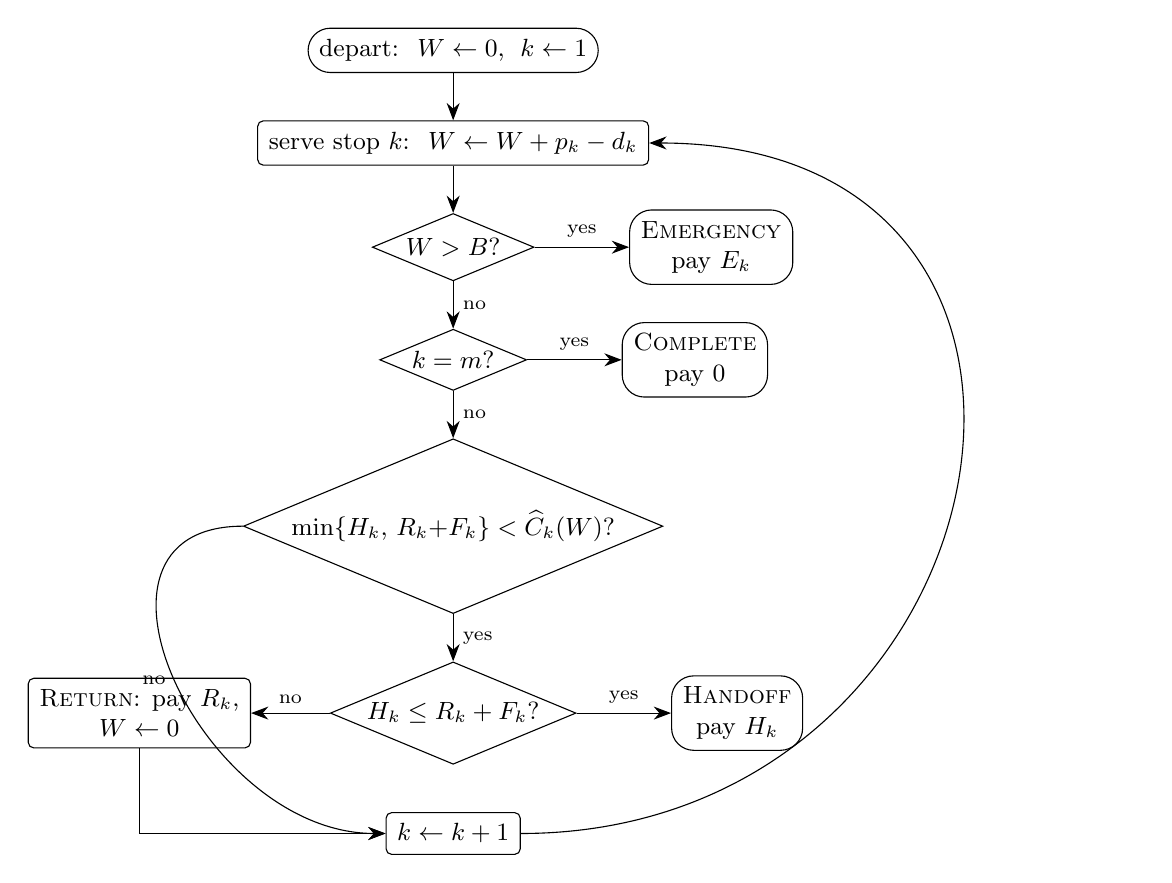
\begin{tikzpicture}[
  node distance=6mm and 8mm,
  box/.style={rectangle, rounded corners=2pt, draw, align=center,
              inner sep=4pt, font=\small},
  dec/.style={diamond, aspect=2.4, draw, align=center, inner sep=1.2pt,
              font=\small},
  term/.style={rectangle, rounded corners=8pt, draw, align=center,
               inner sep=4pt, font=\small},
  arr/.style={-{Stealth[length=2.2mm]}}]
\node[term] (start) {depart:\; $W \gets 0$,\; $k \gets 1$};
\node[box, below=of start] (serve)
  {serve stop $k$:\; $W \gets W + p_k - d_k$};
\node[dec, below=of serve] (guard) {$W > B$?};
\node[term, right=12mm of guard] (emg) {\textsc{Emergency}\\ pay $E_k$};
\node[dec, below=of guard] (last) {$k = m$?};
\node[term, right=12mm of last] (done) {\textsc{Complete}\\ pay $0$};
\node[dec, below=of last] (trig)
  {$\min\{H_k,\, R_k{+}F_k\} < \widehat C_k(W)$?};
\node[dec, below=of trig] (which) {$H_k \le R_k + F_k$?};
\node[term, right=12mm of which] (ho) {\textsc{Handoff}\\ pay $H_k$};
\node[box, left=10mm of which] (rs)
  {\textsc{Return}: pay $R_k$,\\ $W \gets 0$};
\node[box, below=of which] (inc) {$k \gets k + 1$};
\draw[arr] (start) -- (serve);
\draw[arr] (serve) -- (guard);
\draw[arr] (guard) -- node[above, font=\scriptsize]{yes} (emg);
\draw[arr] (guard) -- node[right, font=\scriptsize]{no} (last);
\draw[arr] (last) -- node[above, font=\scriptsize]{yes} (done);
\draw[arr] (last) -- node[right, font=\scriptsize]{no} (trig);
\draw[arr] (trig) -- node[right, font=\scriptsize]{yes} (which);
\draw[arr] (trig.west) to[out=180, in=180, looseness=1.4]
  node[left, font=\scriptsize]{no} (inc.west);
\draw[arr] (which) -- node[above, font=\scriptsize]{yes} (ho);
\draw[arr] (which) -- node[above, font=\scriptsize]{no} (rs);
\draw[arr] (rs) |- (inc);
\draw[arr] (inc.east) to[out=0, in=0, looseness=1.8] (serve.east);
\end{tikzpicture}%
}
\caption{Online decision loop of \textsc{Baton}. After every stop the
policy compares the estimated cost of continuing against the current
prices of the two recourse levers and exercises the cheaper lever only
when continuing is dearer; a depot return resets the load state and the
loop proceeds on the same route.}
\label{fig:flow}
\end{figure}

Two reference points calibrate the empirical results. The
\emph{clairvoyant bound} pays $0$ on $\{T = \infty\}$ and
$\min\{\min_{k<j} H_k,\, E_j\}$ on $\{T = j\}$---the cheapest of any
pre-breach handoff or the breach itself, with a breach at the first stop
leaving no decision epoch; no policy adapted to $(\mathcal F_k)$ pays
less on any path. Because it is defined for the handoff lever, a
policy with the richer menu may legitimately beat it, and in our
experiments \textsc{Baton} does---the cleanest evidence that the action
generalisation has real value. The \emph{plug-in dynamic program}
replaces the isotonic step by quantile-binned conditional means; run
with fifty times \textsc{Baton}'s training data it approaches the exact
solution of the stopping problem and serves as a near-exact yardstick,
while at equal data it is a fair equal-information competitor. We
emphasise a point of method: mixed-integer programming, the exact
technology of the \emph{planning} stage, cannot compactly encode a
non-anticipative multistage stopping rule, so backward dynamic
programming is the correct exact anchor for the \emph{execution} stage;
we use MIP where it belongs, certifying the routing plans beneath all
our experiments (\S\ref{sec:study}).

Figure~\ref{fig:explainer} makes the machinery concrete on one route of
the Hanoi instance introduced below: the fan of simulated load paths
with a demand-spike day highlighted, the fitted continuation cost
crossing the handoff price at stop 2---ten stops before the breach the
reactive policy suffers---and the resulting cost distribution over two
thousand held-out days.

\begin{figure}[t]
\centering
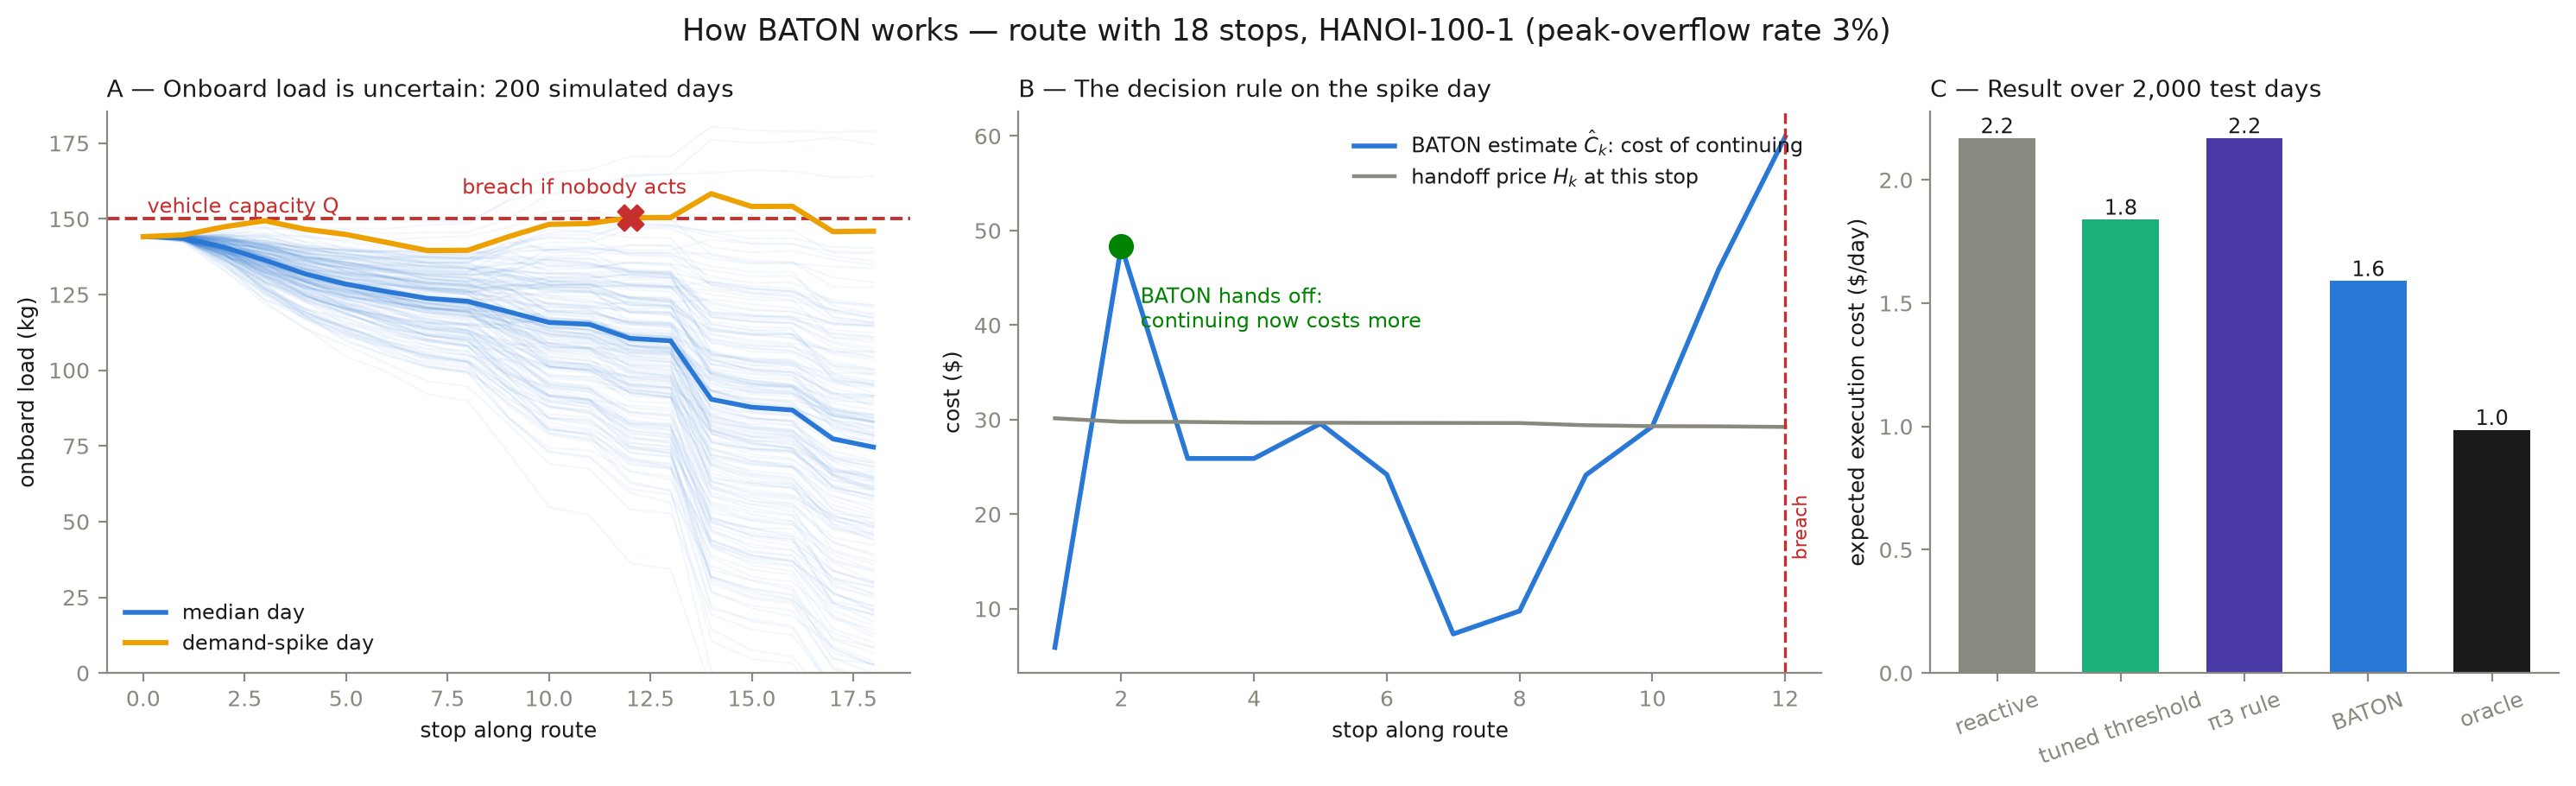
\includegraphics[width=\textwidth]{figures/fig2_how_it_works}
\caption{\textsc{Baton} on one 18-stop route in Hanoi. Left: onboard
load across 200 simulated days; the highlighted day breaches capacity at
stop 12 if nobody acts. Centre: the decision rule on that day---the
estimated cost of continuing $\widehat C_k(W_k)$ crosses the per-stop
handoff price at stop 2, where the policy hands off. Right: expected
execution cost per policy over 2{,}000 held-out days.}
\label{fig:explainer}
\end{figure}


% ══════════════════════════════════════════════════════════════════════
\section{Computational study}\label{sec:study}

Our computational study is designed around a simple discipline: every
claim about the policy must survive a change of environment, a change of
competitor, and a change of yardstick. This section first describes the
environments, competitors, and protocol (\S\ref{sec:setup}), then the
headline comparison across planning regimes (\S\ref{sec:headline}),
the large-scale and real-map benchmarks with the planning-stage
certification (\S\ref{sec:large}), the comparison against learning
methods together with two deliberate negative results
(\S\ref{sec:learning}), and finally the economic and spatial sensitivity
analyses (\S\ref{sec:sensitivity}). All experiments, result files, and
figures are reproducible from a single repository, and every table in
this paper is generated mechanically from the result files.

\subsection{Instances, planners, competitors, and protocol}
\label{sec:setup}

\paragraph{Instances.} Three families are used. The 40 Dethloff
instances \citep{dethloff2001vehicle}, 50 customers each, are the
classical simultaneous pickup-and-delivery benchmark. The Salhi--Nagy
family \citep{salhi1999cluster}, 14 instances of 50--199 customers, is
derived from the CMT instances \citep{christofides1979vehicle} by the
standard coordinate-ratio demand split and extends the size range.
Finally, we introduce a set of instances built on the real drive
networks of Ho Chi Minh City, Hanoi, New York, Paris, and Shanghai
(6\,km radius around the centre, 5{,}800--15{,}800 road nodes per city):
customers are placed at \emph{real shop locations} drawn from
OpenStreetMap's retail layer, snapped to the nearest network node, so
the spatial demand distribution is the city's actual one---market
streets, malls, commercial clusters---and distances are true road
distances \citep{boeing2017osmnx}. Instance sizes reach 400 customers;
Figure~\ref{fig:cities} shows four of the instances with their planned
routes. Demands follow the benchmark protocol (gamma marginals,
coefficient of variation $0.3$, equicorrelated Gaussian copula
$\rho = 0.6$); the city instances use parcel-van magnitudes, with mean
deliveries of 8\,kg, pickup fractions uniform on $[0.2, 0.8]$, and
150\,kg vehicles, which yields the long 12--25-stop routes where
execution policy matters most.

\begin{figure}[tp]
\centering
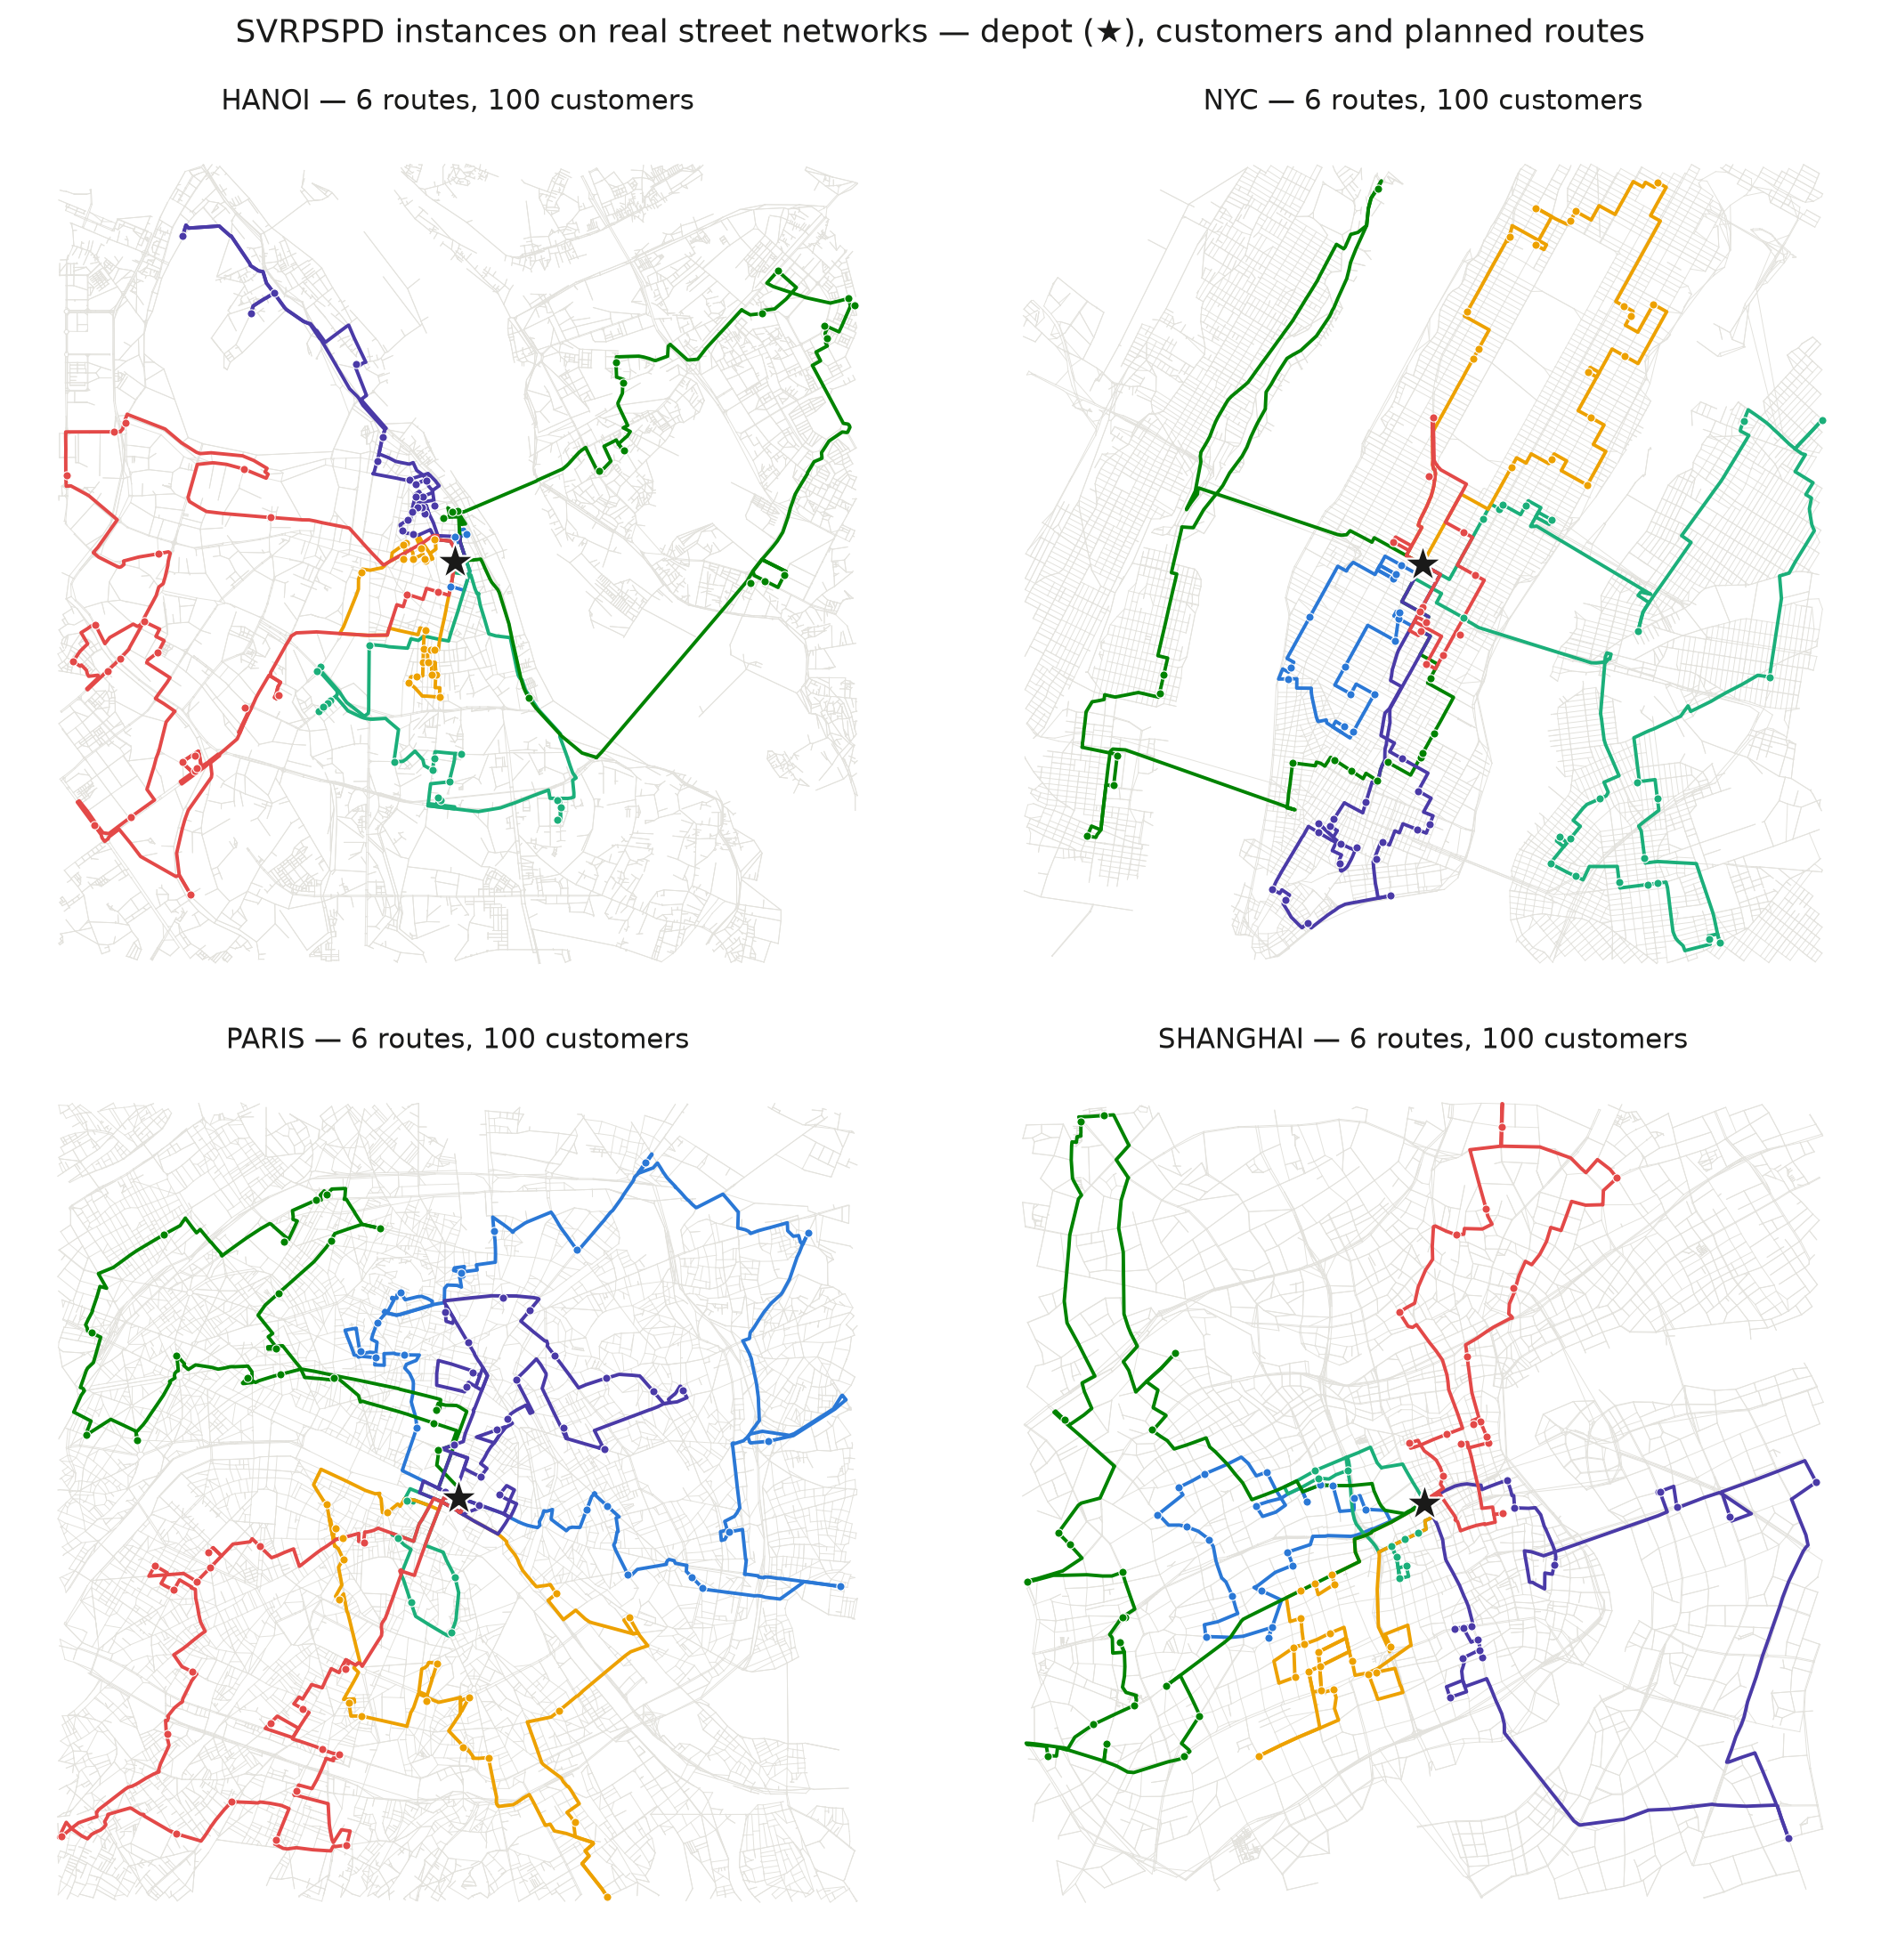
\includegraphics[width=\textwidth]{figures/fig1_city_maps}
\caption{City instances on real street networks, with customers at real
shop locations (Hanoi, New York, Paris, Shanghai; 100 customers each;
depot marked $\star$). Note the true retail clustering---Hanoi's Old
Quarter, Manhattan's commercial spine---that a uniform spatial
convention misses; \S\ref{sec:sensitivity} quantifies its effect.}
\label{fig:cities}
\end{figure}

\paragraph{Planning regimes.} Routes are constructed by an adaptive
large neighbourhood search planner running under six capacity-feasibility
gates of increasing conservatism: a deterministic gate on the nominal
load peak (\textsc{Det}); a sample-average CVaR gate (\textsc{SAA}); a
Wasserstein distributionally robust gate (\textsc{WDRO})
\citep{esfahani2018data}; the quadrant-budget robust gate of
\citet{gounaris2013robust} (\textsc{Rob-G}); a budget-uncertainty gate
in the sense of \citet{bertsimas2004price} (\textsc{Rob-BS}); and a
moment-ambiguity gate in the closed form implied by
\citet{ghosal2024unifying} (\textsc{M-DRO}). Every execution policy is
evaluated on the identical plans of every gate, so planning quality
never contaminates the policy comparison; the plans themselves are
certified in \S\ref{sec:large}.

\paragraph{Competitors.} Eleven execution policies are compared, all
trained (where applicable) on scenarios strictly disjoint from the test
set: the \emph{reactive} policy that never intervenes; the incumbent
endpoint-labelled threshold and its myopic variant, retained as
ablations of Propositions~\ref{prop:bias} and \ref{prop:myopic}; the
\emph{label-corrected tuned threshold} (peak labels, threshold tuned on
realised training cost---the strongest member of the threshold family);
the three published rule-based restocking triggers $\pi_1, \pi_2, \pi_3$
of \citet{salavati2019rule}, adapted to the handoff lever and
grid-tuned on realised cost; a \emph{rollout} policy in the sense of
\citet{secomandi2001rollout}, one step of policy improvement over the
reactive base; a \emph{depot-return restocking} policy in the tradition
of \citet{yang2000stochastic} and \citet{florio2020new}, with real
detour prices and a tuned trigger; \textsc{Baton-ho}, the handoff-only
restriction of our policy; \textsc{Baton} itself; the equal-data
plug-in dynamic program DP$_{N}$; and the near-exact
DP$_{50\mathrm{k}}$. A reinforcement-learning policy re-implemented
from \citet{iklassov2024rl} is compared separately in
\S\ref{sec:learning}, and the clairvoyant bound closes every table.
Table~\ref{tab:competitors} collects the full roster with sources; in
every results table the reported quantity is the expected-recourse
saving relative to the reactive policy, in percent, so \emph{higher is
always better}.

\begin{table}[tp]
\caption{Execution policies compared in this paper. Policies marked
``tuned'' receive their best hyper-parameter by grid search on the
training scenarios; \textsc{Baton} has no tunable parameter.}
\label{tab:competitors}
\centering
\small
\setlength{\tabcolsep}{4pt}
\begin{tabular}{l p{5.1cm} l}
\toprule
Label & Policy & Source \\
\midrule
reactive & never intervenes; emergency on breach & baseline \\
endpoint $+\,\tau$ & endpoint-label threshold (tuned), and its
  myopic variant & ablation (Props.~\ref{prop:bias}, \ref{prop:myopic}) \\
threshold & peak-label threshold (tuned) & strongest threshold ablation \\
$\pi_1$--$\pi_3$ & rule-based restocking triggers (tuned) &
  \citet{salavati2019rule} \\
rollout & one-step policy improvement & \citet{secomandi2001rollout} \\
restock & depot-return restocking, tuned trigger &
  \citet{yang2000stochastic}; \citet{florio2020new} \\
RL & policy-gradient network, GPU-trained &
  \citet{iklassov2024rl} \\
DP$_N$, DP$_{50\mathrm{k}}$ & plug-in dynamic program, equal /
  $50{\times}$ data & \citet{secomandi2009reoptimization} \\
\textsc{Baton-ho} & handoff-only restriction of our policy & this paper \\
\textsc{Baton} & priced-action optimal stopping & this paper \\
oracle & clairvoyant per-day optimum (handoff-only) & upper bound \\
\bottomrule
\end{tabular}
\end{table}

\paragraph{Protocol.} Per route, policies are fitted on $10^3$ training
scenarios and evaluated on $2 \times 10^3$ independent test days;
results aggregate to plan level and then across instances. All
significance statements are paired Wilcoxon signed-rank tests across
plan-level observations. The fleet-economics defaults are
$F_{\mathrm{plan}} = 35$, $F_{\mathrm{sb}} = 20$,
$F_{\mathrm{ho}} = 5$, $c_{\mathrm{tr}} = 3$, $F_{\mathrm{emg}} = 40$,
$s_{\mathrm{ho}} = 1.2$, $s_{\mathrm{emg}} = 2.5$,
$p_{\mathrm{late}} = 1.5$, $p_{\mathrm{breach}} = 10$ (currency units
per vehicle-day or per event; kilometre costs $c_{\mathrm{km}} = 0.1$),
calibrated to the order of magnitude of Southeast-Asian gig-logistics
rates and swept in \S\ref{sec:sensitivity}.

\paragraph{Software.} All planning and execution code is Python 3.11.15
(NumPy 2.4.6, SciPy 1.17.1, pandas 3.0.3); the isotonic regressions of
Algorithm~\ref{alg:offline} use scikit-learn 1.9.0. The MIP
certification of \S\ref{sec:large} solves the two-commodity flow
formulation through PuLP 3.3.2 with Gurobi 13.0.2 as the primary solver
and the open-source HiGHS 1.15.1 as an independent cross-check; both
solvers run single-model with a 300-second budget per instance and
default tolerances. Street networks and shop locations come from
OpenStreetMap via OSMnx 2.1.0 \citep{boeing2017osmnx}, and the
reinforcement-learning baseline is trained with PyTorch on an NVIDIA
T4 GPU. Everything else---the ALNS planner, all six gates, and every
execution policy of Table~\ref{tab:competitors}---is implemented from
the cited papers in plain Python within our repository, so all
competitors share the same simulator, cost model, and data.

\subsection{Headline comparison across planning regimes}
\label{sec:headline}

Table~\ref{tab:grand} reports the central result, and
Figure~\ref{fig:gatedots} draws it. Three observations organise the
discussion.

\begin{table}[t]
\caption{Expected-recourse saving over the reactive policy (\%, mean over
the 40 Dethloff instances) for each planning gate and execution policy
under the three-class fleet cost model; \emph{higher is better}, and the
best non-clairvoyant value per gate is in bold. \textsc{Baton-ho} is the
handoff-only restriction; DP$_{50\mathrm{k}}$ and the clairvoyant oracle
are handoff-only reference points, so \textsc{Baton} may legitimately
exceed them by exercising its richer action set.}
\label{tab:grand}
\centering
\small
\setlength{\tabcolsep}{3.5pt}
\begin{tabular}{l cccc cc cc}
\toprule
& \multicolumn{4}{c}{published / tuned competitors}
& \multicolumn{2}{c}{this paper} & \multicolumn{2}{c}{reference (HO)} \\
\cmidrule(lr){2-5}\cmidrule(lr){6-7}\cmidrule(lr){8-9}
Gate & $\pi_3$ & rollout & restock & threshold & \textsc{Baton-ho} & \textsc{Baton} & DP$_{50\mathrm{k}}$ & oracle \\
\midrule
\textsc{Det} & 17.3 & 20.7 & 5.6 & 24.8 & 26.1 & \textbf{27.8} & 26.5 & 40.7 \\
\textsc{SAA} & 12.8 & 10.0 & 43.7 & 16.6 & 20.5 & \textbf{53.4} & 22.3 & 43.5 \\
\textsc{WDRO} & 7.8 & -4.7 & 34.8 & -8.3 & 9.3 & \textbf{40.9} & 12.0 & 42.0 \\
\textsc{Rob-G} & 15.8 & 9.6 & 43.3 & 17.0 & 21.2 & \textbf{52.8} & 22.9 & 43.5 \\
\textsc{Rob-BS} & 10.8 & 9.5 & 41.0 & 16.6 & 20.7 & \textbf{51.6} & 22.7 & 43.2 \\
\textsc{M-DRO} & 10.0 & -3.1 & 38.8 & -1.8 & 11.9 & \textbf{44.3} & 14.2 & 42.2 \\
\bottomrule
\end{tabular}
\end{table}


\begin{figure}[t]
\centering
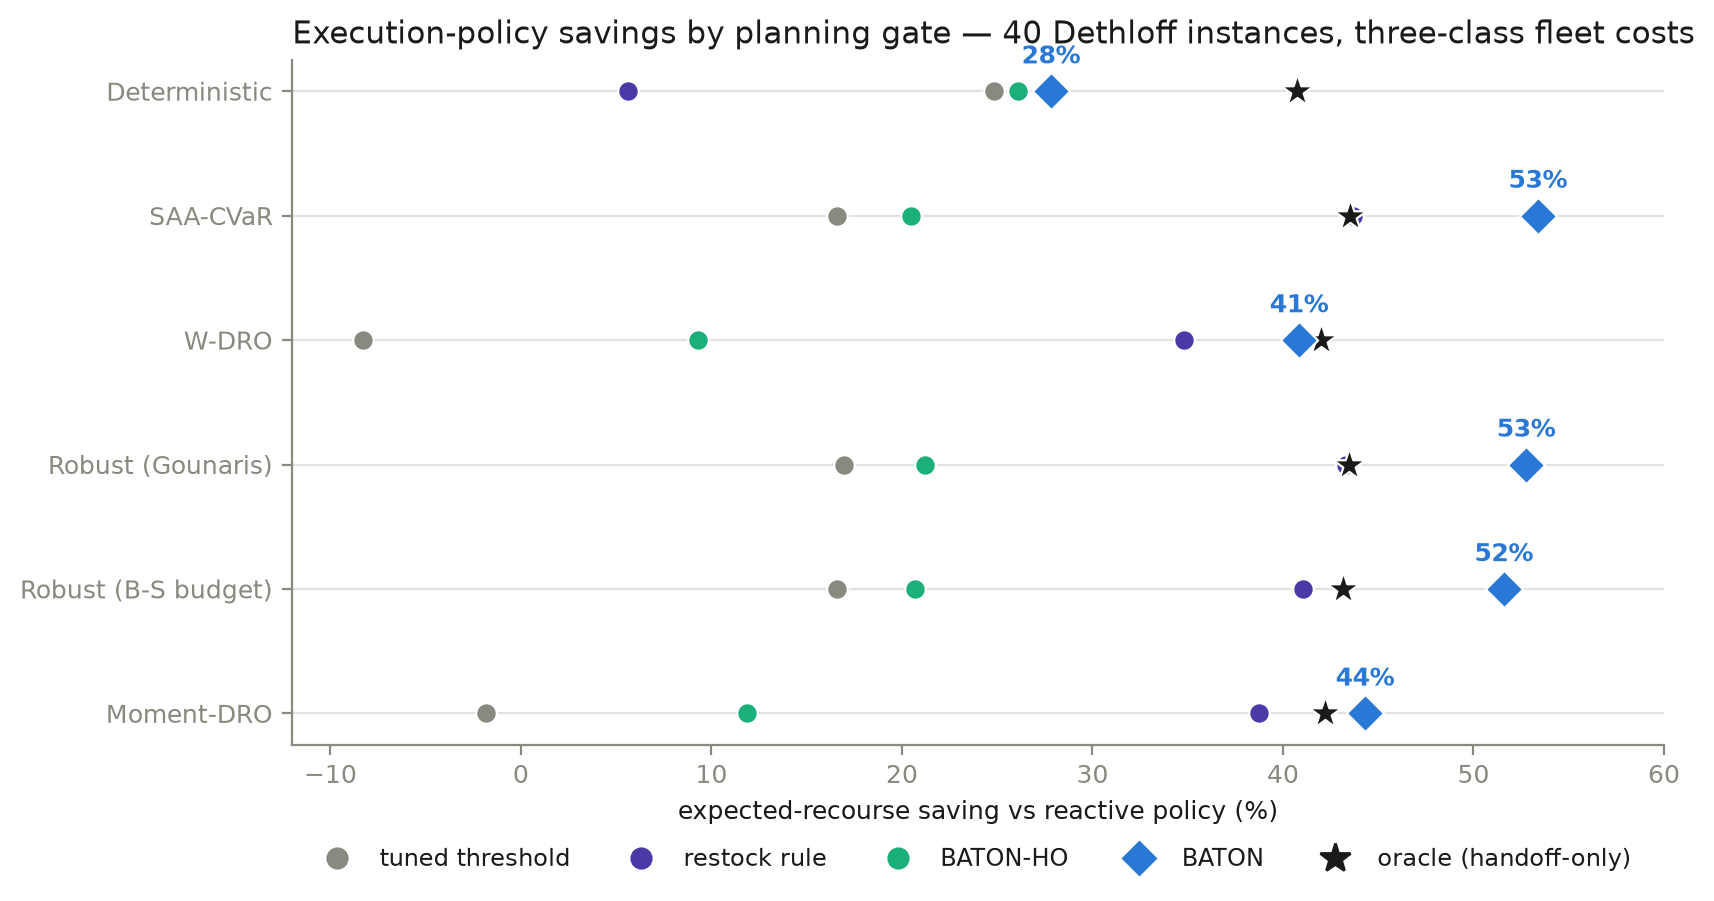
\includegraphics[width=\textwidth]{figures/fig4_gate_dots}
\caption{Expected-recourse saving by planning gate and execution policy
(Table~\ref{tab:grand} drawn). \textsc{Baton} (diamonds) leads on every
gate and exceeds the handoff-only clairvoyant bound (stars) wherever
plans leave slack for the depot-return lever to work with.}
\label{fig:gatedots}
\end{figure}

First, \textsc{Baton} attains the lowest execution cost on every gate,
and the paired tests are unequivocal: against the tuned threshold
\batonWThreshP{} (better on \batonWThreshN{} plan comparisons), against
the strongest rule-based trigger \batonWPiThreeP{}, against the rollout
policy \batonWRolloutP{}, against depot-return restocking
\batonWRestockP{}, against its own handoff-only restriction
\batonWHoP{}, and against the near-exact dynamic program---which sees
fifty times its data but is confined to the handoff lever---%
\batonWDpxlP{} (better on \batonWDpxlN{}).

Second, the \emph{composition} of the win changes across gates in an
instructive way. On the deterministic gate, routes depart packed to
capacity, most breach risk sits at the first stop where no online
policy can act, and all preventive policies compress toward each other;
\textsc{Baton}'s margin there (\svDetBaton{} against \svDetThresh{} for
the tuned threshold) comes mostly from the trigger correction of
Proposition~\ref{prop:myopic}. On every conservative gate---the two
sample-based gates and all three published robust planners---plans
carry slack, breaches happen mid-route, and the depot-return lever
becomes live: \textsc{Baton} roughly \emph{doubles} the saving of the
best handoff-only policy (for instance \svSAABaton{} against
\svSAAHo{} on \textsc{SAA} plans) and \emph{exceeds the handoff-only
clairvoyant bound} (\svSAAOrc{}) on four of the six gates. We emphasise
what that comparison does and does not say: the bound is valid for the
restricted action set, so beating it is not a paradox but a
measurement---of exactly how much the second lever is worth when priced
optimally.

Third, the threshold family collapses where conservatism meets
realistic prices. On \textsc{WDRO} plans the tuned threshold's saving
is \emph{negative} (\svWDROThresh{}): with handoffs carrying their true
standby vehicle-day cost, the thresholds' interventions cost more than
they prevent, while \textsc{Baton} extracts \svWDROBaton{} on the same
plans. A policy that prices actions declines to act when acting has
negative value; a policy that memorises a trigger level cannot.

The synthetic scenarios of Table~\ref{tab:synthetic} isolate the two
defects of \S\ref{sec:defects} under controlled conditions and confirm
Proposition~\ref{prop:bias} at its extremal point: on
collect-then-deliver structure the endpoint-trained policy saves
exactly \ctdVOne{}---it never intervenes---while the label-corrected
policies save half of the reactive cost, and the option-value
correction adds a further margin that grows with route length and the
price ratio.

\begin{table}[t]
\caption{Structural synthetic scenarios (five seeds, $1.2\times10^4$ test
routes each): saving \% over the reactive policy, \emph{higher is
better}. On collect-then-deliver structure the endpoint-labelled
predecessor never intervenes.}
\label{tab:synthetic}
\centering
\begin{tabular}{l ccc}
\toprule
Scenario & endpoint + $\tau$ & peak + $\tau$ & \textsc{Baton-ho} \\
\midrule
collect-then-deliver & 0.0 & 49.2 & \textbf{51.9} \\
milk run, regime switching & 58.9 & 58.9 & \textbf{63.8} \\
milk run, $C/\omega = 20$ & 85.5 & 85.5 & \textbf{88.2} \\
\bottomrule
\end{tabular}
\end{table}


\subsection{Scale, real maps, and certified plans}\label{sec:large}

Table~\ref{tab:large} extends the comparison to the Salhi--Nagy family
and the city instances. On Salhi--Nagy, whose 50--199-customer routes
are tight and long, the picture of the conservative Dethloff gates
repeats at scale: \textsc{Baton} saves \svSalhiBaton{} of reactive
cost---beyond the handoff-only oracle (\svSalhiOrc{})---with the
depot-return lever doing heavy work on the centrally-located depots of
the CMT geometry. On the city instances the same policy correctly
reverses itself: real urban depots sit at the retail centre of gravity
but detours through congested networks are long, the return lever
rarely pays, deployment selection switches it off on most routes, and
\textsc{Baton} equals its handoff-only restriction within noise
(\svCityBaton{} across \nCity{} instances) rather than paying the
estimation cost of a useless action. We regard this
do-no-harm behaviour as a first-class experimental result: an
operator can enable the full menu everywhere and trust the policy to
discover, per route, which levers its geography supports.

\begin{table}[t]
\caption{Large-scale benchmarks under the fleet cost model
(Det-gate plans; saving \% vs.\ reactive, \emph{higher is better};
the proposed policy is in bold, DP$_{50\mathrm{k}}$ and the oracle are
reference points). Salhi--Nagy instances carry
50--199 customers; the city instances (100--400 customers) place
customers at real OSM shop locations on the road networks of Ho Chi Minh
City, Hanoi, New York, Paris and Shanghai, and the uniform twins use the
same cities and demands with uniformly scattered customers.}
\label{tab:large}
\centering
\small
\setlength{\tabcolsep}{4pt}
\begin{tabular}{l r cccccc}
\toprule
Benchmark & $n$ & restock & threshold & \textsc{Baton-ho} &
\textsc{Baton} & DP$_{50\mathrm{k}}$ & oracle \\
\midrule
Salhi--Nagy & 14 & 26.6 & 37.6 & 42.3 & \textbf{53.0} & 42.9 & 49.0 \\
City, real shops & 19 & 0.3 & 10.1 & 10.7 & \textbf{10.8} & 12.4 & 36.8 \\
City, uniform & 9 & 0.5 & 11.3 & 11.9 & \textbf{12.1} & 13.2 & 36.2 \\
\bottomrule
\end{tabular}
\end{table}


Figures~\ref{fig:replay} and~\ref{fig:fleet} put these aggregates back
on the map, using the same rendering of the real road network on which
the instances were built; every trail in both figures follows the actual
shortest road path between consecutive stops, so what is drawn is what
the per-stop price schedules of \S\ref{sec:setting} price.
Figure~\ref{fig:replay} replays the demand-spike day of
Figure~\ref{fig:explainer} on the Hanoi network. The planned vehicle
(solid trail) works outward from the depot while its fitted continuation
cost climbs with the accumulating pickups; at the circled stop the
estimate crosses the handoff price and \textsc{Baton} calls the standby
vehicle, which completes the dashed remainder of the route. The red
cross marks where the reactive policy, facing the identical demands,
instead runs the vehicle to overflow---mid-route, far from the depot,
at the position where the emergency transfer is priced highest and the
largest number of downstream customers is kept waiting.
Figure~\ref{fig:fleet} widens the lens from one route to an entire
200-customer plan on the same network: thirteen vehicles run
simultaneously under \textsc{Baton} through one shared high-demand day.
Seven routes hand off mid-route (circles; the standby vehicle continues
on the dashed trail in the route's colour), two absorb demand spikes
too abrupt for any profitable anticipative action and fall through to
the emergency guard, and the remaining four complete unaided. The
figure makes the operating regime of the policy concrete: recourse is
not an exceptional disaster response but a routine, priced re-balancing
of work across the fleet, exercised on roughly half the routes of a
hard day at a total recourse bill of a few hundred dollars.

\begin{figure}[tp]
\centering
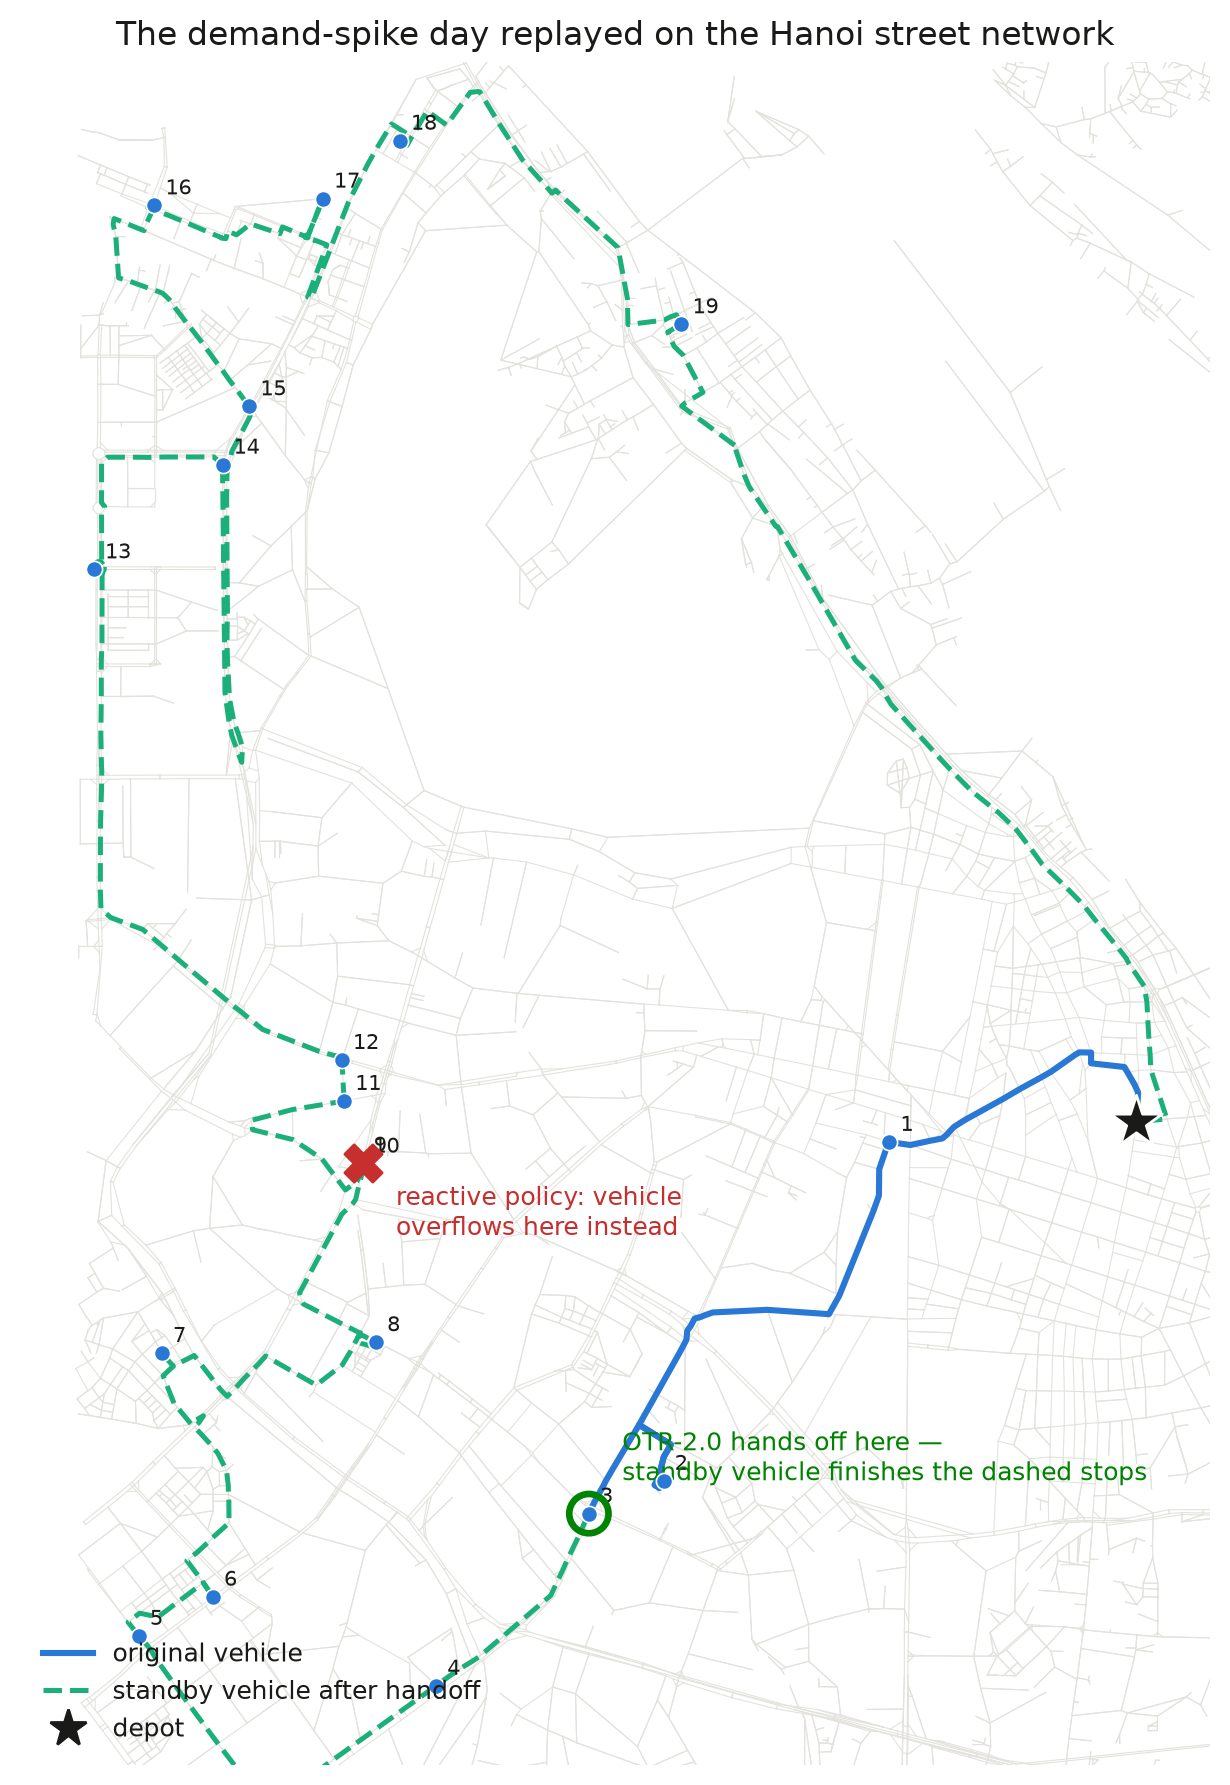
\includegraphics[width=0.92\textwidth]{figures/fig3_map_replay}
\caption{The demand-spike day of Figure~\ref{fig:explainer} replayed on
the Hanoi street network (instance \textsc{Hanoi}-100-1; grey lines are
the OSM drive network, the star is the depot, and every trail follows
real shortest road paths). The planned vehicle drives the solid route;
at the circled stop \textsc{Baton}'s estimated cost of continuing
exceeds the handoff price and a standby vehicle takes over the dashed
remainder. Under the reactive policy the same vehicle continues and
overflows at the red cross, triggering the surge-priced emergency
transfer with the rest of the route still unserved.}
\label{fig:replay}
\end{figure}

\begin{figure}[tp]
\centering
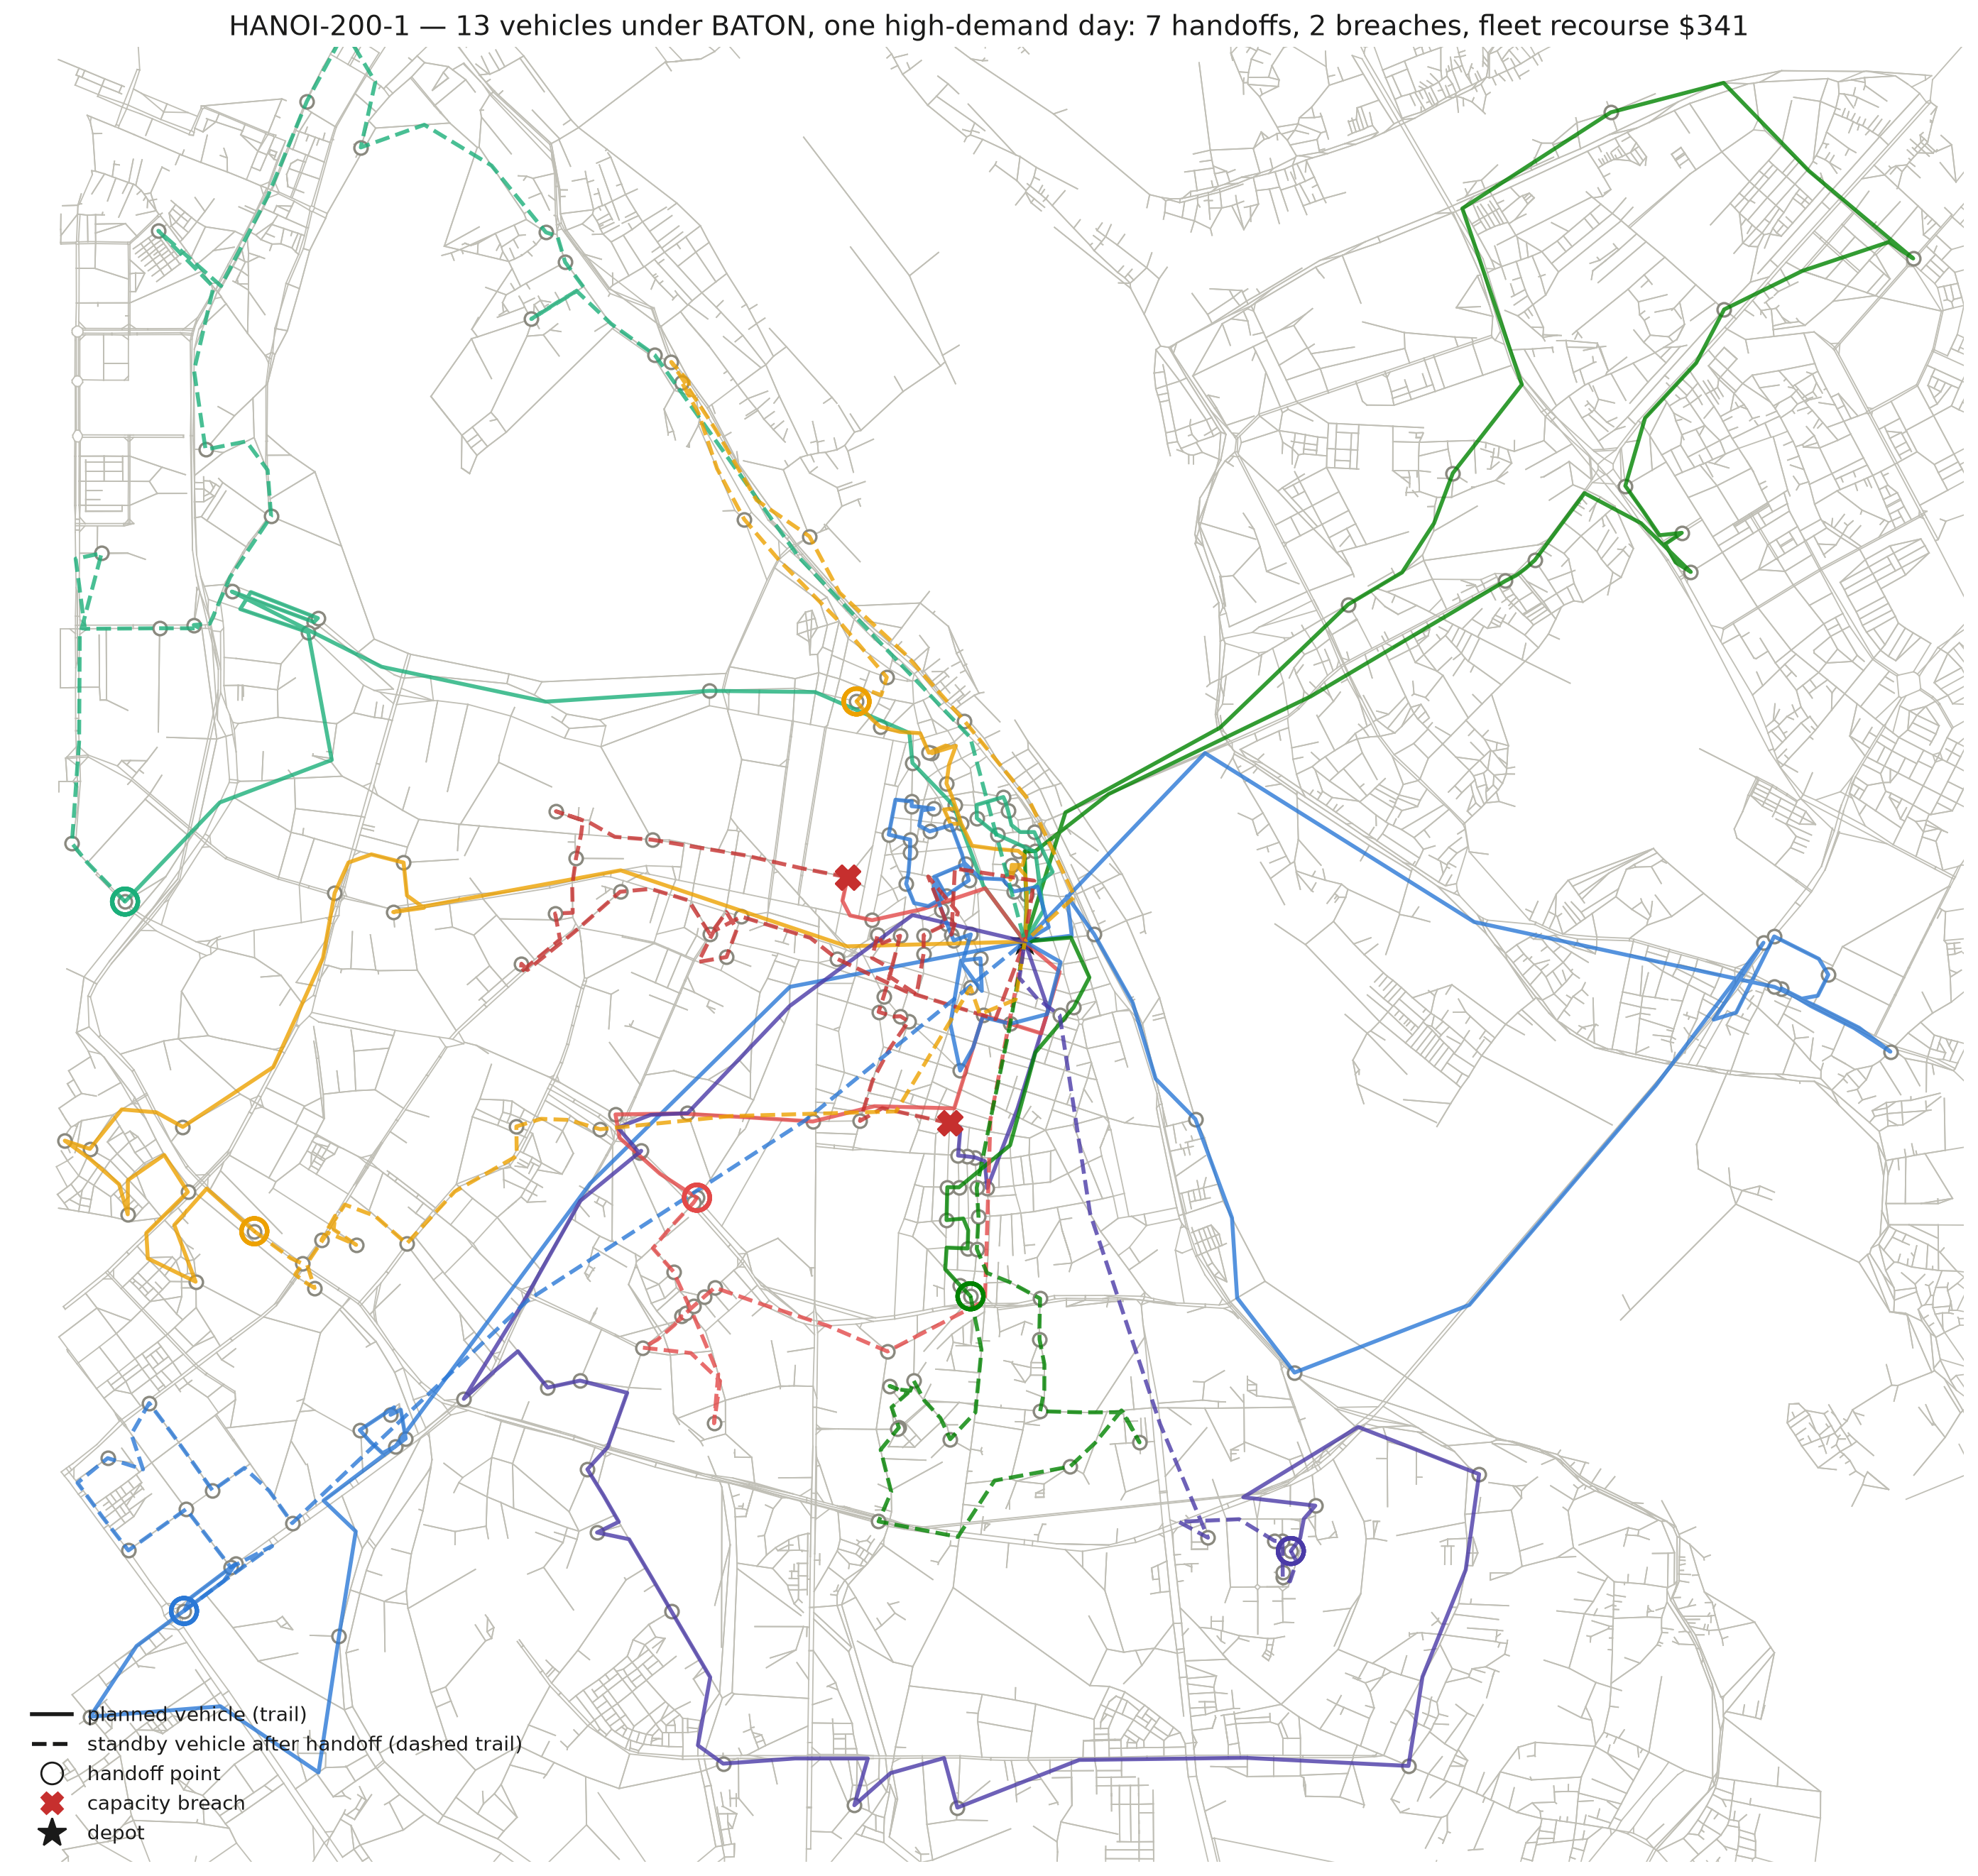
\includegraphics[width=0.92\textwidth]{figures/fig6_fleet}
\caption{One high-demand day for a full 200-customer plan on the Hanoi
network (instance \textsc{Hanoi}-200-1): thirteen vehicles execute
simultaneously under \textsc{Baton}, sharing one demand scenario. Solid
trails are planned vehicles, dashed trails the standby vehicles that
take over at the circled handoff points, and red crosses the two spikes
that outran any profitable anticipative action and fell through to the
emergency guard. Seven of thirteen routes exercised the handoff lever;
the whole day's recourse bill is \$341.}
\label{fig:fleet}
\end{figure}

The routing plans beneath every number above were certified against
mixed-integer programming bounds, using the two-commodity flow
formulation of \citet{montane2006tabu} solved by Gurobi with a
300-second budget per instance. The dual bounds certify the ALNS plans
within \certGap{} of optimality on average (worst case
\certGapMax{}), and at equal time budgets the solver's own incumbents
beat the heuristic plans on only \certBeatN{} instances---so the
execution-stage comparisons run on plans that are simultaneously
near-optimal and representative of what strong planning practice
produces. On 12--24-customer sub-instances, where the MIP proves
optimality outright, even the fast construction heuristic used for the
largest instances lands within 1.2--3.6\% of the optimum.

\subsection{Against learning methods: a GPU-trained policy and two
deliberate negative results}\label{sec:learning}

Because \textsc{Baton} is itself a learned policy, the natural
challenge is a more flexible learner. We re-implemented the
reinforcement-learning approach of \citet{iklassov2024rl}---a policy
network over the observable state (position, load, slack, price ratios,
remaining-demand moments), trained by REINFORCE with a moving
baseline---and trained it on a GPU over the identical routes and
training scenarios available to \textsc{Baton}, evaluating both on
identical held-out days. Table~\ref{tab:rl} reports the outcome. The
learned policy is respectable, clearly beating the rule-based family,
but its best configuration---after quadrupling the training epochs,
adding entropy regularisation, and selecting over learning rates and
seeds---saves \rlBest{} against \textsc{Baton-ho}'s \rlBatonHo{} on the
same days, losing on \rlWinN{} routes (\rlWinP{}). The seeds cluster
within a percentage point of each other, so the gap is not
under-training; it is sample efficiency. A policy-gradient method must
discover the value structure that the backward induction computes
directly, and at a thousand paths per route the regression wins---at
five orders of magnitude less compute.

\begin{table}[t]
\caption{Reinforcement-learning baseline (re-implementation of the policy
architecture of Iklassov et al., 2024) versus \textsc{Baton-ho} on the
identical 50 routes and out-of-sample test days; saving \% vs.\ the
reactive policy, \emph{higher is better}. The learned policy is
trained on a GPU; \textsc{Baton} fits in milliseconds per route on a CPU.}
\label{tab:rl}
\centering
\begin{tabular}{l c}
\toprule
Policy & saving vs.\ reactive (\%) \\
\midrule
40 epochs (paper spec) & 27.6 \\
150 epochs, seed 0 & 27.7 \\
150 epochs, seed 1 & 28.6 \\
150 epochs, seed 2 & 28.7 \\
\midrule
\textsc{Baton-ho} & \textbf{33.9} \\
\bottomrule
\end{tabular}
\end{table}


Two further experiments were designed to fail, and did, in ways that
sharpen the method's justification. First, we enriched the conditioning
statistic beyond the scalar $W_k$ with exactly the features a
representation-learning critique would demand: the precision-weighted
residual that is the posterior location of the day's common demand
factor, the last increment, and the running maximum increment, fitted
with monotonicity-constrained gradient-boosted trees. On 25 real routes
the enriched policy \emph{lost} to the scalar isotonic policy on 23,
by 3.2\% of cost on average, while fitting orders of magnitude slower:
at operational sample sizes the extra features buy more estimation
variance than signal, and Proposition~\ref{prop:monotone}'s shape
constraint is doing the statistical heavy lifting. Second, the
equal-data plug-in dynamic program---the same backward induction with
quantile bins in place of the isotonic projection---collapses exactly
where data are scarcest relative to risk (on conservative plans it
saves nothing or worse; Table~\ref{tab:grand}), because bins cannot
pool information across the load axis the way the monotone projection
can. Together the two null results locate \textsc{Baton} at a
complexity sweet spot: one scalar statistic, one shape constraint, no
free parameters.

\subsection{Economic and spatial sensitivity}\label{sec:sensitivity}

A recourse policy earns its keep only if its advantage survives changes
in the prices that define it. Table~\ref{tab:costsens} and
Figure~\ref{fig:costsens} sweep the four managerial cost levers one at
a time around the defaults: the standby day rate, the emergency
callout, the surge multiplier, and the per-customer lateness price.
\textsc{Baton} leads in every configuration, but the instructive
content is \emph{how}. When standby capacity is dear
($F_{\mathrm{sb}} = 35$), the threshold family collapses to
\dearSbThresh{}---its handoffs cost more than they save---while
\textsc{Baton} holds \dearSbBaton{} by shifting its mix toward depot
returns, ending far above the handoff-only clairvoyant bound
(\dearSbOrc{}). When lateness is expensive, depot returns lose their
appeal and the mix shifts back toward handoffs. No parameter changes
across these worlds; the policy simply re-prices its levers.

\begin{table}[t]
\caption{Sensitivity of the recourse saving (\%) to the fleet-economics
parameters, one factor at a time around the defaults (12 Dethloff
instances, \textsc{Det} and \textsc{SAA} gates). \textsc{Baton}
re-balances its action mix as prices move and leads in every
configuration.}
\label{tab:costsens}
\centering
\footnotesize
\setlength{\tabcolsep}{4pt}
\begin{tabular}{l ccccc}
\toprule
Configuration & restock & threshold & \textsc{Baton-ho} &
\textsc{Baton} & oracle (HO) \\
\midrule
baseline & 24.6 & 20.7 & 23.3 & \textbf{40.6} & 42.1 \\
cheap emergencies ($F_{\mathrm{emg}}{=}25$) & 22.5 & 13.5 & 17.6 & \textbf{39.5} & 31.1 \\
dear emergencies ($F_{\mathrm{emg}}{=}60$) & 32.3 & 35.7 & 39.1 & \textbf{54.4} & 55.4 \\
cheap standby ($F_{\mathrm{sb}}{=}10$) & 28.2 & 37.0 & 41.3 & \textbf{51.3} & 57.7 \\
dear standby ($F_{\mathrm{sb}}{=}35$) & 28.0 & 7.3 & 12.4 & \textbf{41.9} & 24.8 \\
low SLA price ($p_{\mathrm{late}}{=}0.5$) & 33.1 & 22.3 & 27.0 & \textbf{48.8} & 42.0 \\
high SLA price ($p_{\mathrm{late}}{=}3$) & 23.3 & 28.5 & 32.2 & \textbf{46.1} & 47.6 \\
mild surge ($s_{\mathrm{emg}}{=}1.5$) & 26.8 & 20.3 & 24.9 & \textbf{44.2} & 40.3 \\
heavy surge ($s_{\mathrm{emg}}{=}4$) & 29.8 & 30.2 & 33.6 & \textbf{51.4} & 49.3 \\
\bottomrule
\end{tabular}
\end{table}


\begin{figure}[t]
\centering
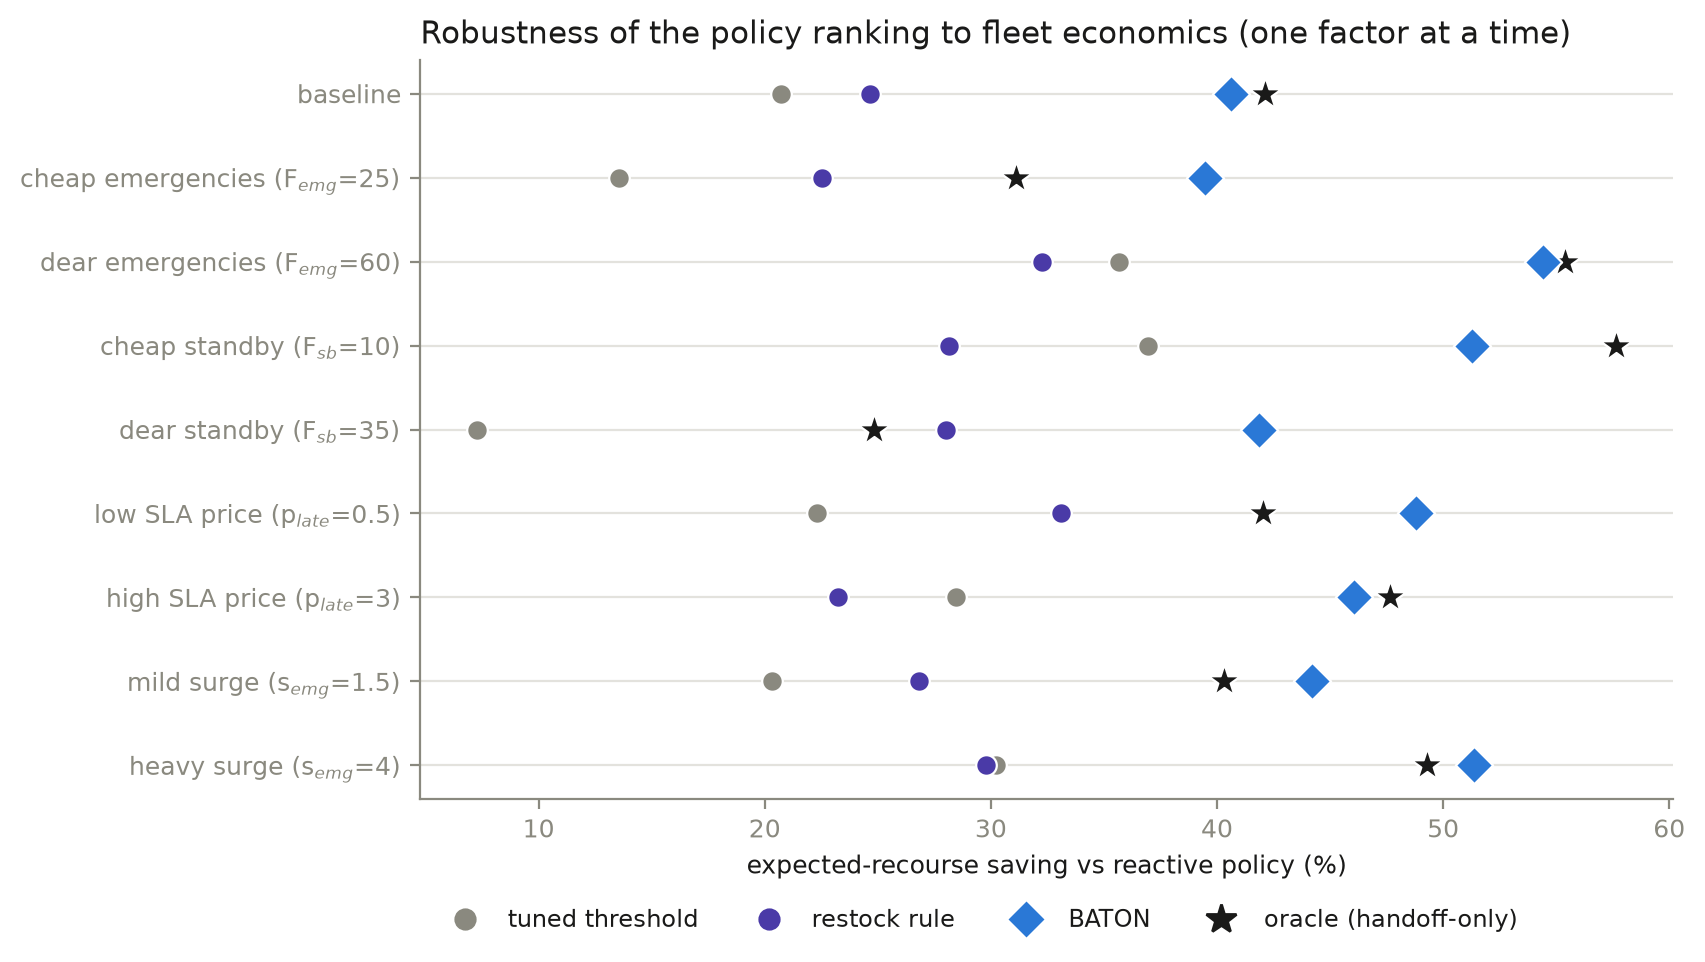
\includegraphics[width=\textwidth]{figures/fig5_costsens}
\caption{Sensitivity of the policy ranking to the fleet economics, one
factor at a time. \textsc{Baton} (diamonds) leads in every
configuration, re-balancing between handoffs and depot returns as the
relative prices move.}
\label{fig:costsens}
\end{figure}

The spatial-structure experiment closes the study. For each city
instance we generated a twin with identical demands and identical seeds
but customers scattered uniformly over the street network rather than
placed at real shops; Figure~\ref{fig:shops} shows the pair for the
200-customer Hanoi instance, and the visual difference is the
experiment: real retail concentrates around the commercial core while
the uniform convention spreads demand into residential and peripheral
blocks. The real retail clustering shortens optimal
routes by \shopTravelSaving{} on average---uniform spatial conventions
materially overstate travel in urban simultaneous pickup-and-delivery
---while the execution-policy ranking and \textsc{Baton}'s margins are
unchanged between the twins. The policy conclusions of this paper do
not depend on where customers stand; the absolute economics do, which
is precisely why we report both.

\begin{figure}[tp]
\centering
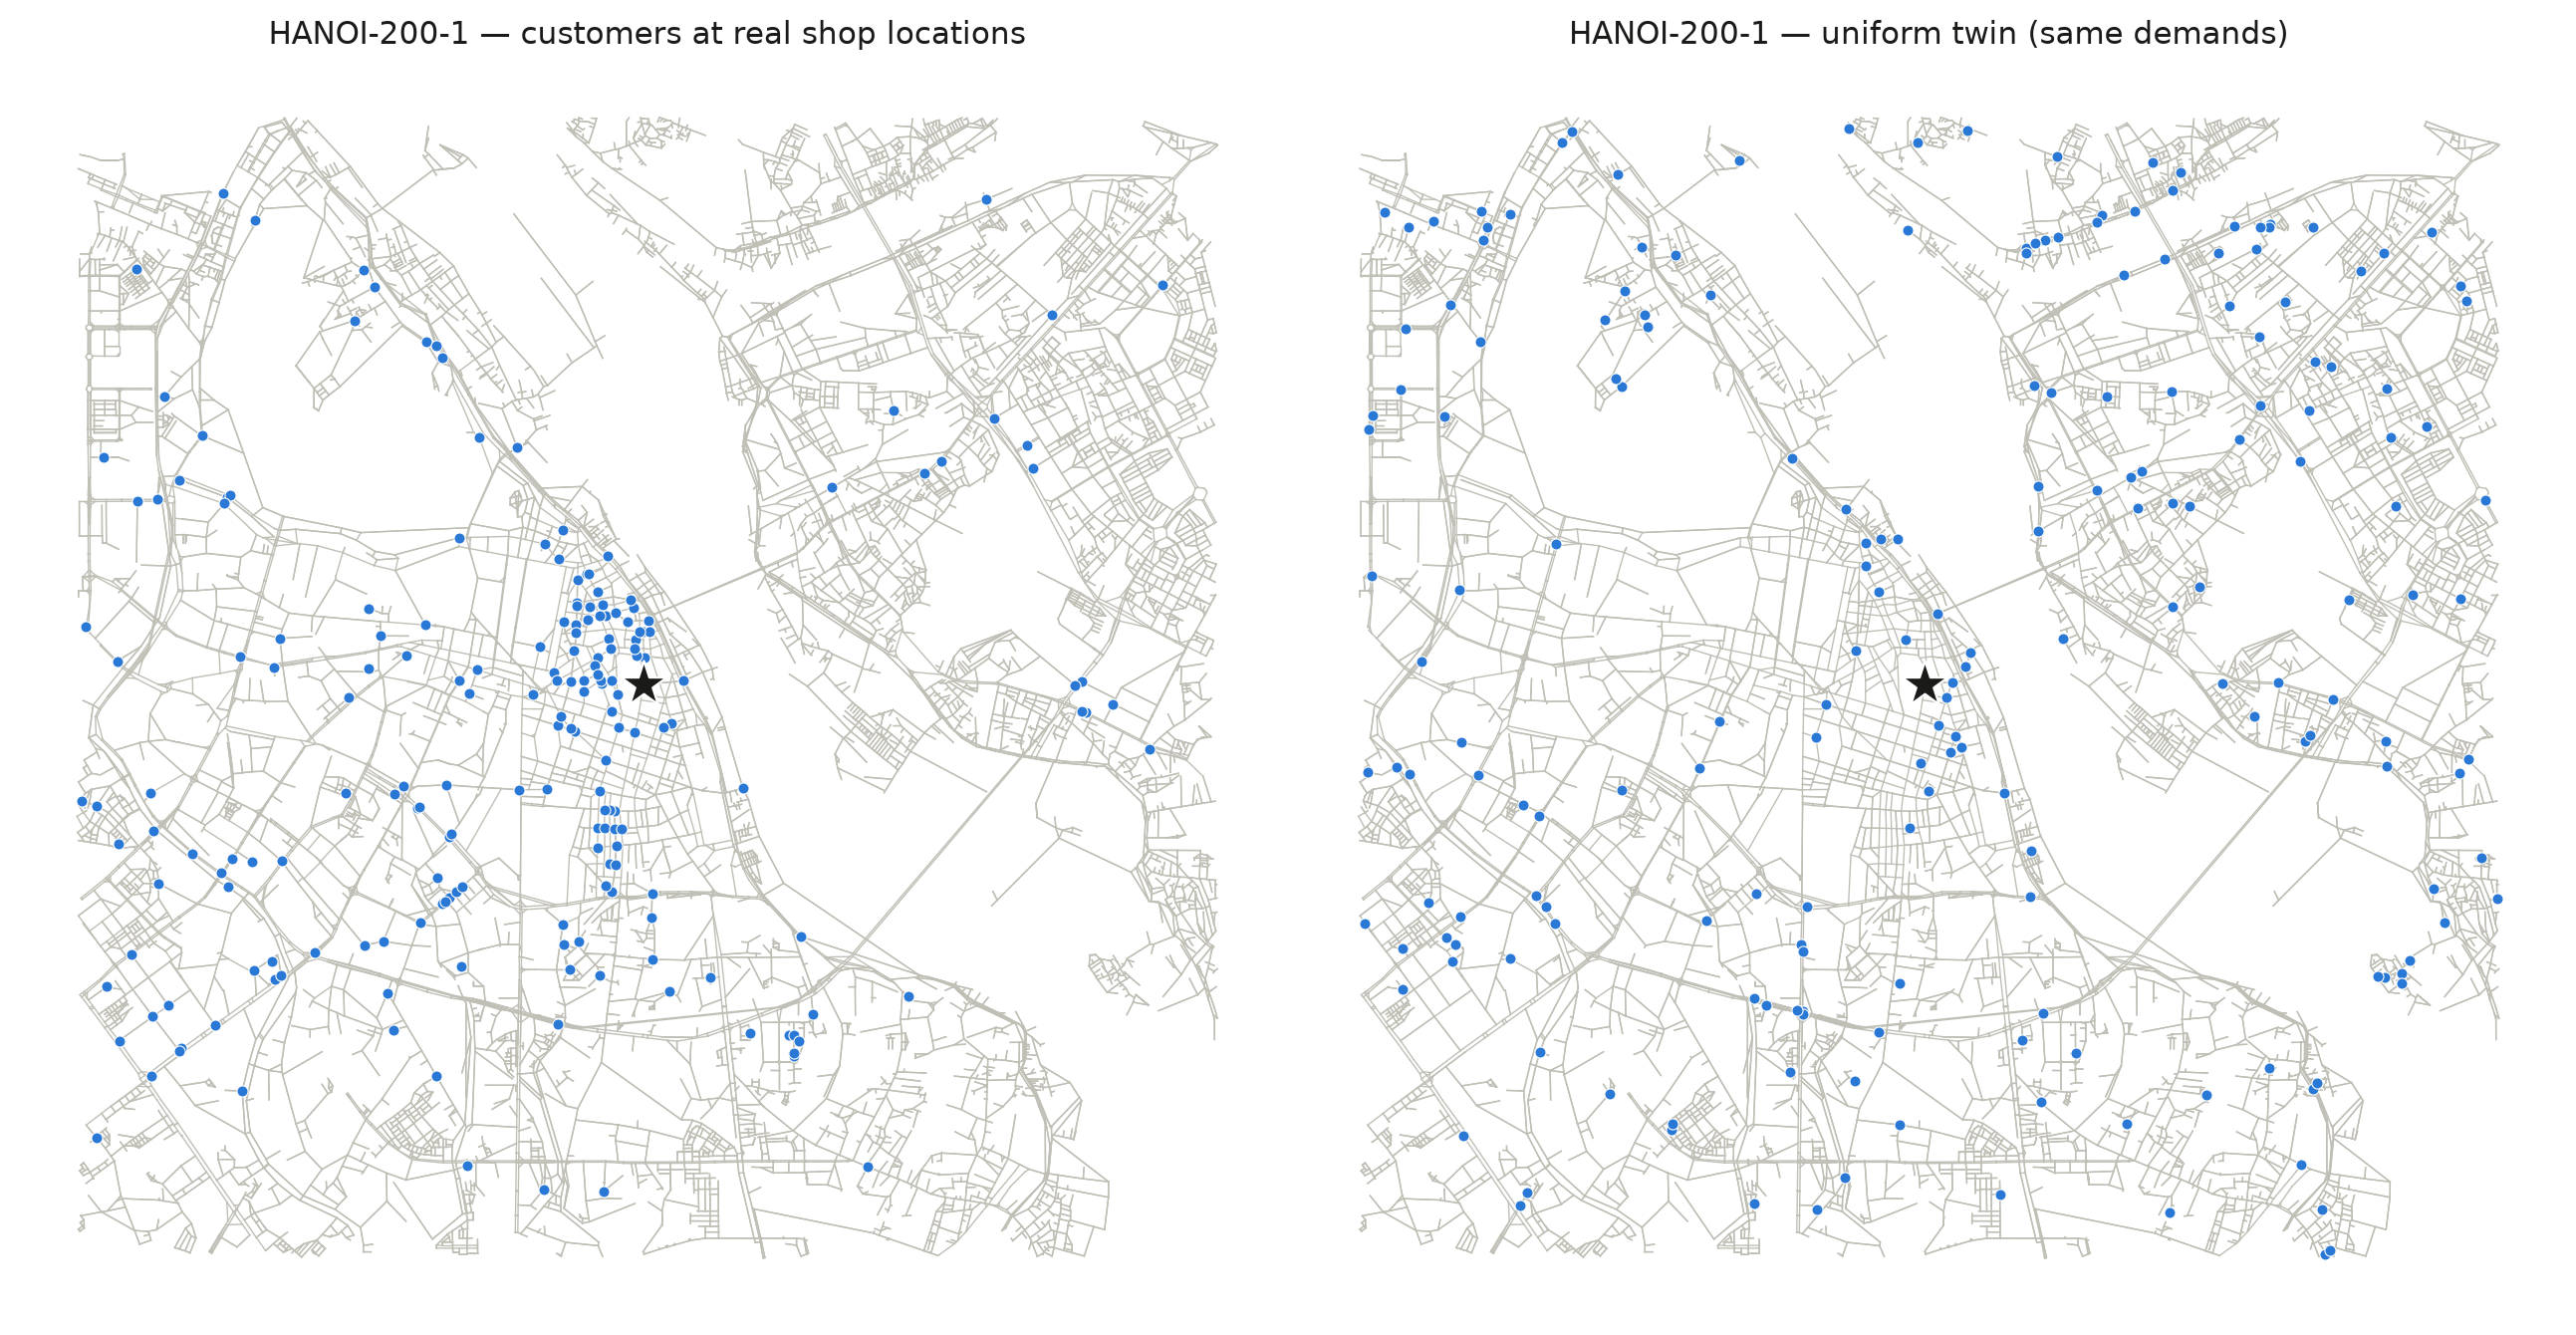
\includegraphics[width=\textwidth]{figures/fig7_shops_vs_uniform}
\caption{The spatial-structure twins for \textsc{Hanoi}-200-1 on the
OSM drive network (star: depot). Left: the 200 customers at real
OpenStreetMap shop locations, clustered along the retail corridors
around the commercial centre. Right: the uniform twin---identical
demand draws, customers scattered uniformly over the same street
network. Real clustering shortens optimal routes by
\shopTravelSaving{} on average while leaving the execution-policy
ranking unchanged.}
\label{fig:shops}
\end{figure}


% ══════════════════════════════════════════════════════════════════════
\section{Managerial insights and conclusions}\label{sec:conclusion}

This paper set out from an operational nuisance---mid-route capacity
breaches in simultaneous pickup-and-delivery---and arrived at a general
prescription for execution-stage recourse: \emph{price the levers,
estimate the cost of waiting, and compare}. The resulting policy,
\textsc{Baton}, is a data-driven optimal-stopping rule that fits in
milliseconds per route from ordinary historical demand logs, carries no
tuning parameter, and accommodates whatever recourse menu an operation
actually offers. Across six planning regimes, three benchmark families
including instances built on real road networks and real retail
locations, and eleven competitors spanning the rule-based,
restocking, rollout, dynamic-programming, and reinforcement-learning
traditions, it delivered the lowest execution cost everywhere,
approached a near-exact dynamic program given fifty times its data, and
exceeded the clairvoyant bound of the single-lever policy class
wherever plans left room for its second lever to work.

For the practitioner, four findings travel beyond our test bed. First,
\emph{label on the peak}. Aggregated per-route data invite risk labels
computed from end-of-route totals, and Proposition~\ref{prop:bias}
shows the resulting policies can be blind to the very event they are
meant to prevent; monitoring must record the running maximum. Second,
\emph{thresholds over-trigger by construction}. The one-sided error of
Proposition~\ref{prop:myopic} means every tuned trigger level buys its
simplicity with premature interventions, and the cost of that
simplicity explodes precisely when intervention prices are high---in
our sweeps the threshold family destroyed value on conservative plans
while the priced policy still earned double-digit savings. Third,
\emph{planning conservatism and execution intelligence are
substitutes, but asymmetric ones}: robust plans leave little recourse
cost to save, yet what remains is recovered almost exclusively by the
policy that prices the full action menu. An operator choosing between a
more conservative planner and a smarter execution layer should note
that the latter kept earning when the former had nothing left to give.
Fourth, \emph{geography selects the lever}. Depot returns dominate
where depots are central---classical benchmark geometries flatter them
---and are nearly worthless on real urban networks with peripheral
depots; a deployed policy must discover this per route, and
\textsc{Baton}'s train-set deployment selection does so at no risk to
performance where the extra lever is useless.

The study has limits that chart the next steps. The policy conditions
on a scalar load statistic; our negative result shows richer statistics
do not pay at a thousand training paths, but fleets with vastly longer
logs may cross that boundary, and the recursion accepts any regressor.
The action set, while general in form, was instantiated with two
levers; partial handoffs---transferring only the riskiest remaining
customers---compose naturally with the same backward induction and
await a per-customer cost model. The demand model treats days as
exchangeable; systematic seasonality would enter through
day-type-specific fits. Finally, our deepest structural finding cuts
toward planning: on deterministically packed routes most breach risk
sits at the first stop, where no execution policy can act, so the
larger prize is a planner whose acceptance gate internalises the fitted
execution cost itself---co-optimising the routes with the recourse
policy that will execute them. The machinery developed here, cheap
enough to sit inside a planner's inner loop, makes that co-optimisation
a concrete and, we believe, imminent possibility.

\ifanon\else
\section*{Acknowledgements}
The author thanks colleagues at British University Vietnam for helpful
discussions.
\fi

\section*{Data availability}
All instance generators, result files, and code sufficient to reproduce
every table and figure are available in a public repository
\ifanon (anonymised for review; link supplied to the editors)\else at
\url{https://github.com/vinhqdang/stochastic_vrp}\fi.

\bibliographystyle{elsarticle-harv}
\bibliography{references}

\end{document}
